\documentclass[a4paper, draft]{article}
\pagestyle{headings}


\title{An introduction to Thermodynamics}

\usepackage{amsmath,amsthm, amsfonts,amscd, amssymb, a4}
\usepackage[final]{graphicx}
\usepackage[final]{listings}
\usepackage{bbm}
\usepackage{empheq}
\usepackage{caption}
\usepackage{tikz}
\usepackage{hyperref}


\renewcommand\lstlistingname{Algorithm}
\captionsetup[lstlisting]{singlelinecheck=false, margin=0pt, font={sf},labelsep=space,labelfont=bf}



% Numbering

%\numberwithin{section}{chapter}
%\numberwithin{equation}{chapter}

% Theorem environments

%% \theoremstyle{plain} %% This is the default
\newtheoremstyle{own}
    {3pt}                    % Space above
    {3pt}                    % Space below
    {\itshape}                   % Body font
    {}                           % Indent amount
    {\scshape}                   % Theorem head font
    {.}                          % Punctuation after theorem head
    {.5em}                       % Space after theorem head
    {}  % Theorem head spec (can be left empty, meaning ‘normal’)
    
\theoremstyle{own}
\newtheorem{thm}{Theorem}[section]
\newtheorem{cor}[thm]{Corollary}
\newtheorem{lem}[thm]{Lemma}
\newtheorem{prop}[thm]{Proposition}
\newtheorem{ax}{Axiom}[section]

%% \theoremstyle{definition}
\newtheorem{defn}{Definition}[section]

%% \theoremstyle{remark}
\newtheorem{rem}{Remark}[section]
\newtheorem*{notation}{Notation}
\newtheorem{algorithm}{Algorithm}[section]
\theoremstyle{remark}
\newtheorem{example}{Example}[section]

% Fix alignments

% \setlength{\parindent}{0cm}

\newcommand*\widefbox[1]{\fbox{\hspace{4em}#1\hspace{4em}}}
\newcommand*\fullbox[1]{\framebox[\columnwidth]{#1}}

%  Math definitions

% Fields
\newcommand{\R}{\mathbb{R}}
\newcommand{\C}{\mathbb{C}}
\newcommand{\Z}{\mathbb{Z}}
\newcommand{\Q}{\mathbb{Q}}
\newcommand{\N}{\mathbb{N}}
\newcommand{\quat}{\mathbb{H}}

%Groups 
\newcommand{\Lo}{\mathbf{O}(3,1)}
\newcommand{\SL}{\mathbf{SL}}
\newcommand{\SU}{\mathbf{SU}}
\newcommand{\Spin}{\mathbf{Spin}}
\newcommand{\Pin}{\mathbf{Pin}}
\newcommand{\SO}{\mathbf{SO}}
\newcommand{\Poincare}{\mathcal{P}}
\newcommand{\Poincarecov}{\widetilde{\mathcal{P}}}
\newcommand{\Poincareprop}{\widetilde{\mathcal{P}}_+^{\uparrow}}
\newcommand{\Aut}{\mathrm{Aut}}

% Rings
\newcommand{\End}{\mathrm{End}}
\newcommand{\CCl}{\mathbb{C}\mathrm{l}}
\newcommand{\Cl}{\mathrm{Cl}}
\newcommand{\Mat}{\mathrm{Mat}}

% Lie algebras

\newcommand{\spin}{\mathfrak{spin}}
\newcommand{\so}{\mathfrak{so}}
\newcommand{\su}{\mathfrak{su}}
\newcommand{\slc}{\mathfrak{sl}}

%Three-vectors
\newcommand{\xt}{\mathbf{x}}
\newcommand{\yt}{\mathbf{y}}
\newcommand{\pt}{\mathbf{p}}
\newcommand{\nt}{\mathbf{n}}
\newcommand{\sigmat}{\mathbf{\sigma}}

% Vector spaces
\newcommand{\Hil}{\mathcal{H}}

% Other
\newcommand{\calE}{\mathcal{E}}
\newcommand{\calD}{\mathcal{D}}
\newcommand{\calF}{\mathcal{F}}
\newcommand{\calP}{\mathcal{P}}
\newcommand{\Fock}{\mathcal{F}}
\newcommand{\Op}{\mathrm{Op}}

\DeclareMathOperator{\per}{per}
\DeclareMathOperator{\sign}{sgn}
\DeclareMathOperator{\logit}{logit}

\begin{document}
\maketitle

\tableofcontents


\section{Microstates and macroscopic quantities}

Suppose that we want to develop a physical model of a gas. Let us assume that this gas consists of a large number of distinguishable particles (molecules) with an identical behavior, that are confined to some volume $V$ which is large compared to the size of an individual particle, but finite (and might in fact change over time), for instance because the gas is contained in a vessel. Then, one approach to describing the state of this physical system could be to record, at any point in time, the exact position and momentum of each of the particles.

If we know how the particles interact with each other and with the vessel, then we could, at least in theory, calculate the future state of the system at any point in time given its state at an initial time. This state is called the {\em microstate} of the system.

However, it is obvious that, given the large number of particles in a gas, this approach is in reality useless - we will never be able to actually calculate all the interactions, and even if we had a very powerful computer that could do this, we would not be able to measure the position and momentum of all particles at one specific point in time precisely enough. 

Fortunately, it turns out that in practice, there are some quantities like the temperature, the volume of the gas and its energy, that we can measure and that follow some empirically derived laws. Thus we could describe the gas at some point in time by specifying these quantities only and see how they develop over time. Such a state is called a {\em macrostate}. Formally, we could describe a macrostate as the values of a set of functions defined on the space of microstates, one function for each relevant quantity like the energy or the temperature. 

We know from experience that the quantities that make up such a state can fluctuate over time. If, for instance, we allow two vessels containing hot liquids to exchange heat, then the temperatures within these vessels will change over time. At some point, however, the system will reach a state called a {\em thermal equilibrium state} and these quantities will settle to certain values and remain constant until we make a modification to the system.

Some of these quantities, like the number of particles or the volume, are {\em extensive quantities}: when we split our system into subsystems (which are still assumed to be large compared to the microscopic scale), these quantities add up. Other macroscopic quantities like the temperature and the pressure do not have this property. However, from what follows, we will see that these are in a certain way derived quantities and that it is useful to start our description of these systems with extensive quantities.

Let us now assume that we have, once and for all, picked a set of extensive quantities like the energy $U$, the number of particles $N$ and the volume $V$, that we combine into a vector
$$
X = (U,V,N)
$$
that we use the fully specify the macroscopic state of our system. Now consider a situation where we have two initially separated systems, say $\Sigma_1$ and $\Sigma_2$, that are in equilibrium and hence, $X$ is constant over time for each of them if seen in isolation. Let us now bring these two systems together and wait until equilibrium is reached again. Then, we know, as we did assume our macroscopic variables to be extensive, that the energy, number of particles and the volume of the new system in total is simply the sum of the individual quantities. But obviously, the values for the individual systems will have changed. If, for instance, we allow two systems, one with a very high temperature and one with a low temperature, to exchange energy, we expect that in the equilibrium state, the first system will have lost some of its energy which has been absorbed by the second system. So how can we find the new values of $X$ for each of the systems? The answer is closely related to the concept of thermodynamical entropy.

\section{Entropy}

One way to introduce the entropy is using a maximum principle - we want to be able to characterize those states that are actually realized after reaching equilibrium as the macrostates that maximize a certain function. Following 
\cite{Callen}, section 1.10, we phrase the assumption that such a function exists as follows (this is in fact a combination of postulate II and postulate III in \cite{Callen})

{\em There exists a function - the entropy - of the extensive parameters of any composite system defined for all equilibrium states with the following property: the values assumed by the extensive parameters in the equilibrium state of an isolated system in the absence of an internal constraint are those that maximize the entropy among all states allowed by the external constraints. Moreover, the entropy is additive with respect to subsystems. It is differentiable and a (strictly) monotonically increasing function of the total energy}.
	
In \cite{Callen}, it is not explicitly mentioned that the maximum principle that is expressed by this statement is only valid for isolated systems, though this becomes apparent from the context. However, we will see later that this restriction is in fact necessary (cf. for instance chapter 9 of \cite{Sweden}). A system can, for instance, reduce its entropy by transferring heat to a system with lower temperature, but this process will inevitably increase the entropy of the composite system. In many practical applications, the composite system is made up by the system under interest and some concieved system acting as the environment that essentially represents the total surroundings of the system under investigation, or - if you want - the entire universe outside of our primary system.

To understand how this principle relates to the famous {\em second law of thermodynamics}, let us consider a hypothetical system consisting of a barrel with a movable wall separating the barrel into two compartments, and assume that the two chambers contain gases with different pressures. Initially, the movable wall is somehow fixed, so that the system has an additional constraint fixing the volumes of the two chambers. Some time after this system has been initially established, the gases inside the two chambers and with them the composite system will have reached equilibrium and the entropy has settled to a certain value. 

When we now allow the wall to move freely, we have effectively removed a constraint. The current state of the system is then obviously still allowed by the remaining constraints, but additional states (i.e. values of the extensive parameters) become accessible. In addition, the system is now no longer in equilibrium. Instead, the wall will start to move until the pressures on both sides are equal and the system settles in a new equilibrium. Our maximum principle assures that the new entropy is maximized in this state. As the initial state was also permissible by the constraints, the new value of the entropy can thus not be smaller than the initial value. In other words, the entropy has increased or remained equal, which is exactly what the second law of thermodynamics states. 

Also note that strictly speaking, the formalism that we are about to develop only assumes the existence of the entropy for equilibrium states. While the wall in the above example is moving, the system is not in equilibrium, so strictly speaking the entropy of the composite system is not even defined during this time. If you think of the states of the system as points in the {\em configuration space} spanned by the extensive parameters, then intuively speaking, the system will disappear from the configuration space if it moved out of equilibrium, for instance due to some interaction with another system or due to some constraints being altered, and only reappear once it has settled into its new equilibrium. We know that the entropy of this new state is equal to or higher than the entropy of the starting point, but we have lost track of the states of the system while the change took place.

To rectify this, it is common to consider only quasi-static processes, i.e. processes that proceed so slowly that at every point in time, the system is actually in equilibrium. Then the process can be described as a path in configuration space, and we can apply calculus or the idea of infinitesimal changes which we will do heavily in what follows. Note, however, that this is an idealization which however turns out to provide a good approximation to many real processes (see also the discussion in section 4.2 of \cite{Callen}).

To see the postulates in action and understand entropy further, let us now conduct a thought experiment. Assume that we have two systems that are initially isolated against each other and against the environment and that each of the subsystems is in equilibrium. As the two subsystems cannot interact, the composite system will then also be in equilibrium and will be characterized by extensive quantities like volume, energy and number of particles.

We now bring together the two systems such that they are connected by a thin, but rigid wall that allows heat to pass, but cannot be crossed by any particles. As soon as this happens, the system is no longer in equilibrium. In fact, energy in the form of heat can now be exchanged between the systems. We have effectively removed a constraint, i.e. the constraint that the individual energies are fixed, but we still have the constraint imposed on us by the conservation of energy, i.e. the sum of the energies remains constant. Thus the energies of the subsystems will change until the composite system has again reached an equilibrium state that we want to determine.

To apply the principle of maximal entropy, we first have to define a system of coordinates for our configuration space, i.e. a set of extensive parameters of the system such that their combined value characterizes the system completely. The choice of these coordinates system and the associated state space is crucial. In particular, we need to define how we reflect the existing constraints. In our case, a possible choice would be to use the individual energies $U_i$ along with the individual particle numbers $N_i$ and the volumes $V_i$. However, if we do this, we still have a constraint, namely $U_1 + U_2 = U$, where $U$ is the total energy of the system that we assume to be a constant. This would restrict the possible trajectories of the system in the configuration space to a submanifold. It is easier to adjust coordinates a bit to better reflect this, so we choose $U, U_1, N_1, N_2, V_1$ and $V_2$. Then the entropy is a function on the configuration space, i.e.
$$
S = S(U_1, V_i, N_i)
$$
More generally, given an arbitrary composite system, one usually choses the total energy $U$ and some extensive parameters of the systems, denoted by $X_i$, as coordinates for the configuration space. If the energies of all but one subsystem is among the $X_i$, then we can reconstruct all energies, and the conservation of total energy is expressed as the simple constraint $U = const$.

 
To extract useful information from the principle of maximum entropy, we now have to relate the total entropy to the entropies of the two subsystems, and this is were the assumption that the entropy is additive comes into play. Specifically, in this example,
we have an entropy $S^i$ for each of the subsystems, and additivity implies that
$$
S(U_1, N_i, V_i) = S^1(U_1, N_1, V_1) + S^2(U - U_1, N_2, V_2)
$$
Let us now see what happens if we allow heat to flow between the systems. The principle of maximal entropy tells us that those parameters which are no longer restricted will then settle at a value which maximizes the entropy. In our case, the parameter $U_1$ is now free to change, and so are the $N_i$ and the $V_i$. Thus, as function of $U_1$, the entropy will be maximized. Thus
$$
0 = \frac{\partial S}{\partial U_1}
$$
at the point of equilibrium. This directly translates into 
$$
0 = \frac{\partial S^1}{\partial U_1}(U_1, N_1, V_1) - \frac{\partial S^2}{\partial U_2}(U - U_1, N_2, V_2)
$$
So the partial derivative of the entropy with respect to the energy seems to control the flow of heat. We call
$$
\beta = \frac{\partial S}{\partial U}
$$
the {\em inverse temperature} and 
$$
T = \frac{1}{\beta}
$$
the {\em temperature} of the system. Note that this is a partial derivative of the entropy and therefore a function of $U, V$ and $N$. Thus we find that stability is reached when the temperatures of both systems reach the same value - a very appealing result. 

What happens to the entropy in the process of reaching equilibrium? Initially, the entropy is the sum $S^1 + S^2$ of the initial entropies of the individual systems. Our postulate states that after equilibrium has been reached, the entropy will be maximal among all possible states that are compatible with the still existing external constraints. As the initial distribution of the energies is clearly compatible with these constraints, we can conclude that the new entropy is at least $S_1 + S_2$, i.e. the total entropy can change in the course of this process, but can never decrease. This is known as the {\em second law of thermodynamics}. Be careful, however, as this is only true for the total entropy - the entropy of an individual subsystem can actually decrease over time.

As part of our postulates, we have assumed that the derivative of $S$ with respect to $U$ is positive, and therefore we can express $U$ as a function of $S$ (and the fixed values for $V$ and $N$). Then of course 
$$
\frac{\partial U}{\partial S} =  (\frac{\partial S}{\partial U})^{-1} = \frac{1}{\beta} = T
$$
When we also take the usual assumption that the entropy is strictly concave, then
$$
\frac{\partial \beta}{\partial U} = \frac{\partial^2 S}{\partial U^2} < 0
$$
and we can therefore invert $\beta$ as a function of $U$, in other words, if, for fixed $N$ and $V$, we know $T$, then we know $U$ and vice versa.

Similary, we can find a physical interpretation for the other partial derivatives. For instance, taking the total derivative of 
$$
S(U(S,V,N), V, N) = S
$$
with respect to $V$ - which is zero as the entropy has a minimum at the equilibrium state - gives 
$$
0 = \frac{d}{dV} S(U(S,V,N), V, N) = 
\frac{\partial S}{\partial U} \frac{\partial U}{\partial V} + 
\frac{\partial S}{\partial V}  
$$
so that we obtain
$$
- \frac{\partial U}{\partial V} = T \frac{\partial S}{\partial V}  
$$
This quantity is called the {\em pressure} and denoted by $P$:
$$
P = - \frac{\partial U}{\partial V} = T \frac{\partial S}{\partial V}  
$$
Finally, what is called the {\em chemical potential} is given by
$$
\mu = \frac{\partial U}{\partial N} = - T\frac{\partial S}{\partial N} 
$$
(see \cite{Callen}, chapter 2). These quantities are called {\em intensive quantities}. As the entropy is assumed to be homogeneous, they do not change if we pass to a subsystem, i.e. the temperature and pressure of a part of a system are equal to the temperature and pressure of the full system (in equilibrium). As the fundamental relations that we have derived so far will appear over and over again in thermodynamics, let us summarize them once more before moving on.

\begin{empheq}[box=\widefbox]{align*}
	T &=  \frac{1}{\beta} = (\frac{\partial S}{\partial U})^{-1}  \\
	P &= - \frac{\partial U}{\partial V} = T \frac{\partial S}{\partial V}   \\
	\mu &= \frac{\partial U}{\partial N} = - T\frac{\partial S}{\partial N} 
\end{empheq}
So the temperature describes how the energy depends on the entropy, the pressure measures how it depends on the volume and the chemical potential measures the contribution of the particle number to the energy.

This simple example can be generalized as follows. Suppose we have an entropy presented as a function 
$$
S = S(U, X_1, \dots, X_n)
$$
where the $X_i$ are some arbitrary extensive variables that together with $U$ span the configuration space. We also assume that the total energy is constrained to a specific value $U_0$ but that the other parameters can vary freely (implicitly, we therefore make the assumption that the configuration is an open subset of $\R^{n+1}$  so that we can apply calculus or at least has a non-empty interior). The maximum entropy principle can then be phrased conveniently in terms of differentials and the Hessian. In fact, the entropy is a smooth function which has a differential $dS$, and so is the coordinate function $U$. If we think of a tangent vector as an infinitesimal variation, then the variations which are compatible with the constraint $U = U_0$ are the tangent vectors in the kernel of $dU$. The maximum entropy principle then states that on the subspace $U = U_0$, the entropy $S$, as a function of the $X_i$, has a maximum. If we assume that this is true for every $U_0$, this implies that, at the equilibrium point, the kernel of $dU$ is contained in the kernel of $dS$ and that the Hessian matrix
$$
{\mathcal H}_{X_i}(S) = (\frac{\partial^2 S}{\partial X_i X_j})_{i,j}
$$
of partial derivatives with respect to the $X_i$ is negative definite.


It is important to realize that macroscopic variables are only defined for systems that are in equilibrium. If we remove an internal constraint,  then, for some time, the system will not be in equilibrium and therefore {\em not} be represented by a point in the configuration space. Once we reach equilibrium, the system "reappears" in the configuration space and will be located at a (nearby, if the change was small) point. In theoretical considerations, we often work with idealized processed which are supposed to be a sequence of small changes to the system such that points in the configuration space given by the equilibrium states are so close to each other that they are reasonably close to a continuous or even smooth curve $\gamma$ in the configuration space, so that we can apply the apparatus of calculus to draw conclusions. This is called a {\em quasi static process}. If we are particularly interested in the state of a specific subsystem, say the first system, we could alternatively work in the configuration space given by $X_1$ and $X$, and observe how the equilibrium states of the composite system move in this space to deduce the changes in $X_i$.


\begin{example}[see 4.1 and 4.4 in \cite{Callen}]\label{ex:idealgascomposite}
Let us now make our example more concrete by assuming a specific relation between entropy and the extensive parameters which holds for both subsystems. Specifically, let us assume that the entropy is given by
$$
S = \bar{S}(V,N) + N C \ln U
$$
with a positive constant $C$, where $\bar{S}$ is a function of volume and particle number alone (we will see later that this is true for an ideal gas). Then, by taking partial derivatives, we find that
$$
\frac{1}{T} = \frac{\partial S}{\partial U} = CN \frac{\partial \ln U}{\partial U} = \frac{CN}{U}
$$
so that we obtain
$$
U = NCT
$$
Note that this holds for both systems, and we also assume that the constant $C$ is the same for both systems. Now let us again assume that at some point, we allow heat to flow between the two subsystems, but keep their volumes and particle numbers constant. We want to compare the entropy before allowing heat to flow and after we have removed the constraint and reached equilibrium again. The initial entropy is the sum of the entropies of both subsystems. The same is true for the final entropy. So the change of the total entropy is the sum of the changes of the individual entropies. In any case, the energy will be preserved, so that, if $T_f$ is the final temperature in which the composite system has settled, we have
$$
U = (N_1 + N_2) C T_f = N_1 C T_1 + N_2 C T_2
$$
In other words, the final temperature is the weighted arithmetic mean of the initial temperatures:
$$
T_f = \frac{N_1 T_1 + N_2 T_2}{N_1 + N_2}
$$
As volume and particle number for each of the subsystems is constant and the energy of each subsystem is proportional to its temperature, the change of the entropy of subsystem $i$ will be given by
$$
\Delta S_i = N_i C \ln \frac{T_f}{T_i}
$$
Note that this is {\em not} necessarily positive, i.e the entropy of a subsystem can decrease. If, for instance, $N_1 = N_2$, then $T_f$ will simply be the mean of the $T_i$, and therefore $T_f > T_i$ for one of the $i$ (unless the initial temperatures are already identical). Then the system $i$ will increase its temperature and its entropy, but the other subsystem will decrease its entropy and its temperature. The important point, however, is that change in the total entropy, given by
$$
\Delta S_1 + \Delta S_2 = C [N_1 C\ln \frac{T_f}{T_1} + N_2 \ln {T_f}{T_2}] 
= C \ln \frac{T_f^{N_1 + N_2}}{T_1^{N_1} T_2^{N_2}}
$$
is positive. And this is always true, as the numerator is guaranteed to be at least equal to the denominator by the inequality of weighted arithmetic and geometric mean, and therefore the logarithm is never negative.
\end{example}

\section{Quasistatic and irreversible processes}

We have already defined a quasistatic process to be a process during which the system is at every point in time in equilibrium so that macroscopic quantities like temperature and pressure are well defined. As this term is often the source of confusion, let us take some more time to discuss this.

One of the reasons why the concept of quasistatic processes can be challenging is that different authors use that term with different meanings. In \cite{Schroeder}, a quasi-static process is first defined in section 1.5 for the special case of a slow compression.

\begin{quote}
I need to assume that as the gas is compressed it always remains in internal equilibrium, so that its pressure is uniform from place to place (and hence well defined). For this to be the case, the piston's motion must be reasonably slow, so that the gas has time to continously equilibrate to the changing conditions. The technical term for a volume change that is slow in this sense is quasistatic.
\end{quote}

So the key point here is that the macroscopic variables are at any point in time well defined, so that it makes sense to speak about temperature and pressure of a system and its entropy (which is usually assumed to be a function of these variables). A bit later, in section 2.6, when reversible and irreversible processes are discussed, Schroeder defines a process to be reversible if its entropy remains unchanged and explicitly points out that while every reversible process is quasi-static (otherwise its entropy would not be well defined) but not every quasi-static process is reversible:

\begin{quote}
	In Chapter 3 I will prove that every reversible volume change must in fact be quasi-static...a quasi-static process can still be irreversible, however, if there is also heat flowing in or out or if  entropy is being created in some other way.
\end{quote}

Unfortunately, some authors use the terms quasi-static and reversible interchangeably. An example is \cite{Sweden}, where Sweden states in section 11.1 that

\begin{quote}
In the limit of infinitesimal steps, the increase of entropy can vanish. Such a series of infinitesimal steps is called a quasi-static process. A quasi-static process is reversible. Since there is no increase in entropy, it could be run backwards and return to the initial state.
\end{quote}

We will not adopt this convention but differentiate between quasi-static processes and reversible processes, as it is done by Schroeder. This is also the approach that Callen takes. In \cite{Callen} section 4.2, he defines a quasistatic process as follows 

\begin{quote}
... a process on the hypersurface [the configuration space - added by the author] .... from an initial state to a terminal state. Such a curve is known as a quasi-static locus or a quasi-static process. A quasi-static process is thus defined in terms of a dense succession of equilibrium states.
\end{quote}

and proceeds to define a process to be reversible when the entropy does not change along the path in configuration space that the process defines, and to be irreversible if the entropy is increased.

In other words, a quasi-static process is a process which can be sufficiently well approximated by a continous (and in fact smooth curve) in the configuration space spanned by the extensive parameters of the system in question. For every point of this curve, the entropy is then well defined, so that we can apply our formalism to make predictions about the behaviour of the system.

Note however that the term "equlibrium states" is to be taken with a grain of salt. To illustrate this, let us again consider the process of heat flowing between a body and a heat bath. Let us denote the variables referring to the heat bath with an index HB. The heat bath and the body under consideration together then form a composite system. Then we can, as we have done it during our discussion of the identification of the temperature with a partial derivative, use additivity to write the entropy of the overall system as
$$
S_{tot}(U_{tot}, U, V_{HB}, V, N_{HB}, N) = S(U, V, N) + S_{HB}(U_{tot} - U_, V_{HB}, N_{HB})
$$
Let us now assume that the temperature of the heat bath $T_{HB}$ is different from the temperature $T$ of the body. Then we have already seen that the overall system will not be in equilibrium, i.e. $dS_{tot} > 0$. If the heat transfer is sufficiently slow, however, for instance because the body and the heat bath are connected by a wall with very low thermal conductivity, then each system considered in isolation, i.e. the body and the heat bath, will be in internal equilibrium. So each of them has a well defined temperature and entropy, and the above equation makes sense. Thus the process defines a curve in the configuration space and would thus have to be considered as quasi-static, even though the overall system is not in equilibrium.

So we need to interpret the term "equilibrium states" in a pragmatic way (and looking at section 4.4 of Callens book, for instance, where he essentially uses the same approach to discuss heat flow, indicates that he did so as well). Note, however, that the overall system has no physically meaningful temperature. Formally, however, we can of course take the partial derivative of the above expression for the entropy and obtain
$$
\frac{\partial S_{tot}}{\partial U_{tot}} = \frac{\partial}{\partial U_{tot}} S_{HB}(U_{tot} - U_, V_{HB}, N_{HB}) = \frac{1}{T_{HB}}
$$
so that formally, the temperature of the overall system is identical to that of the heat bath. Once the system has settled into an equilibrium, this is the same as the temperature of the body and this expression matches our physical intuition. Until then, however, this does not appear to be meaningful - which should not surprise us, as we already know that the temperature as an intrinsic quantity is only physically meaningful if the system is in equilibrium.

Still, we can work with the formula for the entropy and use it to derive predictions. We could, for instance, relate the temperature in equilibrium to the heat capacities of the heat bath and the body, as Callen does it in section 4.4 of \cite{Callen}. It is also instructive to look at the change in total entropy. We have, using the fact that by definition, $T_{tot} = T_{HB}$, 
\begin{align*}
T_{tot} dS_{tot} &= T_{HB} (dS_{HB} + dS)  \\
&= T_{HB} dS_{HB} + (T_{HB} - T) dS + T dS
\end{align*}
The first term represents the heat flowing into the heat bath. The third term represents the heat flowing into the hot body. The second term, however, is an additional contribution to the entropy. If conservation of energy holds for the composite system and no mechanical work is done, then
$$
0 = dU_{tot} = dU_{HB} + dU = T_{HB} dS_{HB}  + T dS
$$
and combining these two equations shows that
$$
T_{tot} dS_{tot} = (T_{HB} - T) dS
$$
So this term represents the excess entropy that is generated due to the heat transfer between two system with different temperatures. We have seen that, unless $T_{HB} = T$, $dS_{tot} > 0$, so this process is irreversible and entropy is created out of nothing.


\section{The energy representation}

So far we have worked with the entropy, considered its derivatives and used them to draw conclusions on equilibrium states. Essentially, we have seen that the entire behavior of the macroscopic variables of a thermodynamical system is governed by the entropy. This is called the {\em entropy representation}. In this representation, the energy $U$ is a variable and the entropy a function on the configuration space.

However, we have also seen that the relation between entropy and energy for given $V$ and $N$ can be inverted, so that we can express the energy as
$$
U = U(S,V,N)
$$
and we have used the chain rule to relate the partial derivatives of $U$ to those of $S$. Clearly, $U$ as a function of $S$ contains the same information, as we can always revert to $S$ as a function of $U$. In many cases, however, it is more convenient to work with the energy as a primary quantity. This is called the {\em energy representation}, and in this representation, the entropy is a coordinate and the energy a function on the configuration space.

Let us now write down the total differential of the energy $U$, as a function of $S, V$ and $N$. Using what we have learned about the partial derivatives of $U$ in the previous section, we find that

\begin{empheq}[box=\widefbox]{align*}
dU = T dS - P dV + \mu dN
\end{empheq}

This equation is so important that it is often referred to as the  {\em fundamental thermodynamic equation}. It corresponds to three different ways to add energy to a system. First, we can exercise mechanical force by decreasing the volume. This will require an amount of work given by
$$
dW = F dx = P A dx = - P dV
$$
We therefore call the quantity (mathematically this is a one-form on the state space)
$$
dW = - P dV
$$
the {\em work } done on the gas. Note that this is in general not a closed one-form and not the total differential of any function $W$, so the notation has to be taken with care. Similarly, we call the one-form
$$
dQ = T dS
$$
the {\em heat}. When we consider a thermodynamical process, i.e. a path in the state space, which leaves the number of particles constant, we then find that
$$
dU = dQ + dW
$$
In other words, the change of energy, assuming a constant number of particles, is the sum of the heat added to the system and the work done on the system. This is the famous {\em first law of thermodynamics}. We note that - as discussed before - our formalism applies only to quasi-static processes, which is why some sources call $T dS$ the quasi-static heat and $- P d V$ the quasi-static work. 

The identification of the transferred heat $dQ $ with $TdS$ can be inverted to arrive at the relation 
$$
dS = \frac{dQ}{T}
$$
To illustrate the power of this seemingly simple relation, let us consider a {\em heat engine} which is a device that can exchange heat with a reservoir at temperate $T_h$ and a second reservoir at a lower temperature $T_l$ in order to produce some mechanical work $W$. This engine is supposed to operate in cycles, so that after one cycle, the state of the engine is restored to its original state. 

Let us assume that during one cycle, the engine consumes a certain amount $Q_h$ out of the reservoir with the higher temperature and transfers some heat $Q_l$ into the reservoir with the lower temperature. As the internal energy of the engine does not change during a cycle, we can conclude that
$$
W = Q_h - Q_l
$$
or 
$$
\frac{W}{Q_h} = 1 - \frac{Q_l}{Q_h}
$$
This quantity is often called the {\em efficiency} of the engine and denoted by $e$. On the other hand, using the form of the first law stated above, we can conclude that the entropy of the first reservoir is decreased by $\frac{Q_h}{T_h}$ while that of the reservoir with the lower temperature is increased by $\frac{Q_l}{T_l}$.
Thus the total change of entropy of the entire system (the engine plus the reservoirs) is
$$
\Delta S = \frac{Q_l}{T_l} - \frac{Q_h}{T_h}
$$
As this is non-negative, we can conclude that
$$
\frac{Q_l}{T_l} \geq \frac{Q_h}{T_h}
$$
or
$$
\frac{Q_l}{Q_h} \geq \frac{T_l}{T_h}
$$
Combining this with our expression for the efficiency, we find that
$$
e = 1 - \frac{Q_l}{Q_h} \leq 1 - \frac{T_l}{T_h}
$$
Thus we have derived a universal upper boundary for the efficiency of a heat engine, without even making any assumptions about the exact nature of the engine or having a closed expression for the entropy. In many cases, however, the entropy can be expressed as an expression of the extensive parameters, either derived from statistical considerations, which we will do in a later chapter, or based on empirical considerations. To illustrate this, let us consider an example.

\section{The model of an ideal gas}

An {\em ideal gas}  is a thermodynamical system which is given by the following fundamental relations:
\begin{align*}
PV &= NRT \\
U &= cNRT
\end{align*}
Here $R$ is the {\em gas constant} which is related to Avogadros number $N_A$ and the Boltzmann constant $k_B$ by $R = N_A k_B$ and $c$ is typically equal to $3/2$. As the {\em heat capacity at constant volume} is given by
$$
c_V = \frac{\partial U}{\partial T}|_V = c N R
$$ 
we see that up to the constant $R$, the number $c$ is the heat capacity of the gas per mole of substance. Also note that the {\em equipartition theorem} relates $c$ to the number $f$ of degrees of freedom by
$$
f = 2c
$$
Let us now see whether we can derive the entropy of the ideal gas from these two fundamental relations. We know that the entropy is homogeneous. Thus we can define an entropy density $s$ by
$$
s(U,V) = S(U,V,N=1)
$$
and have that
$$
S(U,V,N) = N S(\frac{U}{N}, \frac{V}{N}, 1) = N s(\frac{U}{N}, \frac{V}{N})
$$
Of course $s$ has the same partial derivatives with respect to $U$ and $V$ as $S$, and therefore we obtain the following expression for its total differential:
$$
ds = \frac{\partial S}{\partial U} dU + \frac{\partial S}{\partial V} dV
$$
We can express this by the intensive quantities that we have defined and obtain
$$
ds = \frac{1}{T} dU +  \frac{P}{T} dV
$$
Using the fundamental relations above with $N=1$, we have
\begin{align*}
\frac{1}{T} &= cR \frac{1}{U} \\
\frac{P}{T} &= \frac{R}{V} 
\end{align*}
so that
$$
ds = cR \frac{1}{U} dU + \frac{R}{V} dV
$$
and therefore we obtain in a bit of a shorthand notation
$$
ds =  cR d \ln U - R d \ln V
$$
This allows us to find an expression for $s$, namely
$$
s = s_0 + cR \ln \frac{U}{U_0} - R \ln \frac{V}{V_0} = s_0 + R \ln \big[ \big( \frac{U}{U_0} \big)^c \frac{V}{V_0} \big]
$$
with an unknown constant $s_0$, a reference volume $V_0$ and a reference energy $U_0$. 
By multiplying by $N$ again, we find that (note that we need to use $\frac{U}{N}$ and $\frac{V}{N}$ according to the defining relation for $s$)
$$
S = N s_0 + N R \ln \big[ \big( \frac{U}{N U_0} \big)^c \frac{V}{N V_0} \big] = N s_0 + N R \ln \big[ \big( \frac{U}{U_0} \big)^c \frac{V}{V_0} N^{-c - 1}  \big]
$$
If we want, we can now express the unknown constant in terms of the entropy of a reference state - in fact, we find that this is the entropy of a single particle at volume $V_0$ and energy $U_0$. Conversely, if we start with an assumed entropy of this type, we can compute 
$$
\frac{1}{T} = \frac{\partial S}{\partial U} = \frac{cRN}{U}
$$
which gives us
$$
U = cRNT
$$
and similarly 
$$
PV = -TV \frac{\partial S}{\partial V} = TV \frac{RN}{V} = NRT
$$
Thus we can recover the laws of an ideal gas from the entropy. 

For later reference, let us also express the entropy in terms of temperature, volume and particle number. We can use the ideal gas relations to write
$$
\big( \frac{U}{U_0} \big)^c \frac{V}{V_0} N^{-c - 1} = N_0^{-c}  \big(  \frac{T}{T_0} \big)^{c} \frac{V}{V_0}
$$
so that, absorbing $-c R \ln  N_0$ into the constant $s_0$ and splitting the logarithm, we find that
$$
S = N s_0 + c N R \ln \frac{T}{T_0}  + N R \ln \frac{V}{V_0}  
$$

Let us now use the formula that we have found for the entropy to derive a similar expression for the energy $U$.
First, let us calculate the chemical potential $\mu$. The partial derivative of $S$ with respect to $N$ is given by
\begin{align*}
\frac{\partial S}{\partial N} &= \frac{\partial}{\partial N} \big( N s_0 + N R \ln \big[ \big( \frac{U}{U_0} \big)^c \frac{V}{V_0} N^{-c - 1}  \big]  \big)    \\
&= s_0 + R \ln \big[ \big( \frac{U}{U_0} \big)^c \frac{V}{V_0} N^{-c - 1}  \big] + N R \frac{\partial}{\partial N}  \ln \big[ \big( \frac{U}{U_0} \big)^c \frac{V}{V_0} N^{-c - 1}  \big]
\end{align*}
The first two terms are recognized as $\frac{S}{N}$. The last term can be calculated as follows
\begin{align*}
\frac{\partial}{\partial N}  \ln \big[ \big( \frac{U}{U_0} \big)^c \frac{V}{V_0} N^{-c - 1}  \big] &= 
\frac{\partial}{\partial N}   \ln \big[  N^{-c - 1}  \big] \\
&= -(c+1) \frac{\partial}{\partial N}   \ln N = - (c+1) \frac{1}{N}
\end{align*}
Putting all this together yields
$$
\frac{\partial S}{\partial N} = \frac{S}{N} - (c+1) R
$$
When we combine this expression with the definition of $\mu$ as $-T$ times the partial derivative, we obtain
$$
\mu  = -T s_0 - T R \ln \big[ \big( \frac{U}{U_0} \big)^c \frac{V}{V_0} N^{-c - 1}  \big] + (c+1) RT = - T \frac{S}{N} + (c+1) RT 
$$
which we can also write as
$$
\mu N = - T S + c NRT + PV
$$
Taking a look at the equations that we started with, the second term is simply the energy and the third term is $PV$. We therefore find that
$$
\mu N = - TS + U + NRT
$$
or 
$$
U = TS - PV + \mu N
$$
as an expression for the internal energy in terms of entropy, volume and particle number plus the intensive variables temperature, pressure and particle number - which, of course, is exactly the expression predicted by our discussion of homogeneous functions in the appendix.

The ideal gas that we have discussed so far was assumed to only contain one type of substance, so you would call this a {\em monatomic ideal gas}. Let us now see what happens if we consider a mixture of several ideal gases. As the gases do not interact, they will all occupy the same volume $V$, and we also assume equilibrium, so that the gases all have the same temperature $T$. However, each of them will exert a certain pressure $P_i$ on the walls of the vessel in which the gas is contained, called the {\em partial pressure}, and the total pressure is given by
$$
P = \sum_i P_i
$$
a fact which is sometimes called Dalton's law. As we assume that the gases do not interact, the ideal gas laws hold for each of them separately, so that
\begin{align*}
P_i V &= N_i R T \\
U_i &= c_i N_i R T
\end{align*}
Note that the first relation implies that
$$
P_i = N_i \frac{RT}{V} 
$$
and
$$
P = N \frac{RT}{V} 
$$
so that
$$
P_i = \frac{N_i}{N} P
$$
Let us now again derive an equation for the entropy of the mixture. To do this, we start with the relation
$$
TS = U + PV - \sum_i \mu_i N_i
$$
We know that the total energy is the sum of the $U_i$ and the total pressure is the sum of the $P_i$. Thus 
$$
TS = \sum_i U_i + \sum_i P_i V - \sum_i \mu_i N_i
$$
Let us now assume that the chemical potentials of the components are the same as it would be in isolation (which seems reasonable as we think of the components as non-interacting, we will later verify this by showing that the expression for $S$ that we obtain in this way gives the correct gas laws - however we will also justify this more formally a bit later). Thus we assume that
$$
\mu_i = -T s_{0, i} - T R \ln \big[ \big( \frac{U_i}{U_0} \big)^c \frac{V}{V_0} N_i^{-c - 1}  \big] + (c_i+1) RT
$$
Now the ideal gas laws in the form written above imply that
$$
\frac{U}{U_0} = \frac{N_i}{N_0} \frac{T}{T_0}
$$
so that
$$
\big( \frac{U_i}{U_0} \big)^c_i  N_i^{-c_i - 1} = N_0^{-c_i}  \big(  \frac{T}{T_0} \big)^{c_i} \frac{1}{N_i}
$$
By redefining the constant $s_{0,i}$ we can therefore write the chemical potential as
$$
\mu_i = -T s_{0, i} - T R \ln \big[ \big(  \frac{T}{T_0} \big)^{c} \frac{V}{N_i V_0} \big] + (c_i+1) RT
$$
Therefore
$$
N_i \mu_i = - N_i T s_{0, i} - N_i T R \ln \big[ \big(  \frac{T}{T_0} \big)^{c} \frac{V}{N_i V_0} \big] + N_i (c_i+1) RT
$$
Now the last term is
$$
N_i (c_i+1) RT = N_i c_i R T + N_i R T = U_i + P_i V
$$
so that
$$
N_i \mu_i = - N_i T s_{0, i} - N_i T R \ln \big[ \big(  \frac{T}{T_0} \big)^{c} \frac{V}{N_i V_0} \big] + U_i + P_i V
$$
Plugging this into our equation for $TS$ above, the last two terms cancel with $\sum_i U_i$ and $\sum_i P_i V$, and we obtain
$$
TS =  \sum_i N_i T s_{0, i} + \sum_i  N_i T R \ln \big[ \big(  \frac{T}{T_0} \big)^{c} \frac{V}{N_i V_0} \big]
$$
so that the entropy is
$$
S = \sum_i N_i  s_{0, i} + \sum_i  c_i N_i R \ln   \frac{T}{T_0}  +  \sum_i  N_i R \ln \frac{V}{N_i V_0} 
$$
in accordance with the expression in \cite{Callen}, section 3.4. Note that a gas consisting of $N_i$ particles (or moles) of constituent $i$ at temperature $T$ and pressure $P_i$ would occupy the volume
$$
\frac{N_i RT}{P_i} = \frac{N_i RT}{P \frac{N_i}{N}} = \frac{RT}{P} = V
$$
and its entropy would therefore be
$$
 N_i  s_{0, i} +  c_i N_i R \ln   \frac{T}{T_0}  +   N_i R \ln \frac{V}{N_i V_0} 
$$
Therefore we find that {\em the entropy of a mixture of ideal gases} is the sum of the entropies that each constituent would have at particle number $N_i$, temperature $T$ and pressure $P_i$ (or equivalently volume $V$). Put differently, if we think of our system as a composite system where each subsystem has volume $V$, temperature $T$ and consists of all atoms of one type, we could appeal to the additivity of entropy to calculate the entropy of the overall system and would arrive at exactly the same expression. This alternative approach to deriving the entropy also shows that our earlier assumption that the chemical potentials are independent of each other is not only justified but in fact a direct consequence of the additivity of the entropy. Note, however, that for this to work, we need to make sure that the two gases are distinguishable, i.e. that for each molecule we can tell to which gas it belongs, as otherwise our subsystems would not be well defined (see also section 2.6 of \cite{Schroeder} for a discussion of the subtleties related to this).


It is interesting to analyze that expression a bit further. For that purpose, let us imagine that we have a collection of separated gases, each with a particle number $N_i$ and each at the same pressure $P$ and temperature $T$. Let $N$ again denote the total particle number. The volume of each gas is then given by
$$
V_i = \frac{N_i R T}{P} 
$$
and the total volume is 
$$
V = \sum_i \frac{N_i R T}{P}  = \frac{N R T}{P}
$$
The total entropy of the system given by this initially separated collection of gases is then
$$
S_{initial} = \sum_i N_i  s_{0, i} + \sum_i  c_i N_i R \ln   \frac{T}{T_0}  +  \sum_i  N_i R \ln \frac{V_i}{N_i V_0} 
$$
As
$$
\frac{V_i}{N_i} = \frac{V}{N}
$$
this is the same as
$$
S_{initial} = \sum_i N_i  s_{0, i} + \sum_i  c_i N_i R \ln   \frac{T}{T_0}  +  \sum_i  N_i R \ln \frac{V}{N V_0} 
$$
When we now allow the gases to mix, no mechanical work is done as the systems already have the same pressure, and no heat is exchanged, as they already have the same temperature. Once equilibrium is reached, we can apply the formula that we have found above to conclude that the final entropy of the system is
$$
S_{final} = \sum_i N_i  s_{0, i} + \sum_i  c_i N_i R \ln   \frac{T}{T_0}  +  \sum_i  N_i R \ln \frac{V}{N_i V_0} 
$$
The difference between these two terms is given by
$$
\Delta S = S_{final} - S_{initial} = \sum_i  N_i R \ln \frac{V}{N_i V_0}  - \sum_i  N_i R \ln \frac{V}{N V_0} 
$$
which is the same as
$$
\Delta S = \sum_i  N_i R ( \ln \frac{N}{N_i })
$$
This is inherently positive, as $N > N_i$, and represents a gain in entropy that is called the {\em entropy of mixing}. We will meet this term again when we calculate the chemical potential of a solute in a later section.

\section{The principal of minimal internal energy}\label{sec:minimalinternalenergy}

We have seen that in the entropy representation, the principle of maximum entropy allows us to derive statements about the equilibrium states of a thermodynamical system. It expresses the equilibrium state as the maximum of some function on the configuration space.

We also know that the energy representation is fully equivalent to the entropy representation. Thus it appears natural that there is an extremum principle in the energy representation which is equivalent to the principle of maximum entropy. It turns out that this is in fact the case, and that the equilibrium states are those states that minimize the total energy subject to the existing constraints.

To derive this principle, let us again assume that we are given a system by a configuration space with coordinates $U, X_1, \dots, X_n$ in the entropy representation. We do not make any specific assumptions on the $X_i$, thus they could be any parameters of a composite system, including the energies of subsystems, but we assume that they are unconstrained. The entropy is then a function
$$
S = S(U, \{ X_i \})
$$
defined on the configuration space. We also know that the temperature is positive and therefore that everywhere on the configuration space
$$
\frac{\partial S}{\partial U} = \frac{1}{T} > 0
$$
Thus we can apply the implicit function theorem and find - at least locally - a function 
$$
U = U(S, \{ X_i \})
$$
such that
$$
S = S(U(S,\{ X_i \}), \{ X_i \})
$$
Note that the $S$ on the left hand side of this equation is a coordinate of the configuration space in the energy representation, while the $S$ on the right hand side is a function on the configuration space of the entropy representation. In a more neutral notation, the map
$$
U \times \text{id} \colon (s,\{ x_i \} ) \mapsto (U(s, \{ x_i \}), x_i)
$$
is a diffeomorphism which maps the configuration space in the energy representation to the configuration space in the entropy representation.

Now let $\gamma$ be an arbitrary smooth curve in the energy representation, given - in coordinates - by
$$
\gamma(t) = (s(t), \{ x_i(t) \})
$$
and let 
$$
\bar{\gamma}(t) = (u(t), \{ x_i(t) \})
$$
be the corresponding curve in the entropy representation. We write
$$
\gamma(0) = (s_0,\{ x_i(0) \} )
$$
and
$$
\bar{\gamma}(0) = (u_0, \{ x_i(0) \})
$$
and assume that this is an equilibrium point. Moreoever, we assume that
$$
s(t) = s_0
$$
for all $t$. We want to show that $U \circ \bar{\gamma}$ has a minimum at $t  = 0$. Differentiating the relation
$$
s(t) = S(\bar{\gamma}(t))
$$
gives 
\begin{align}
\label{eq:chainruleapplied}
0 = \dot{s}(t) =  \langle dS, (\dot{u}(t), \{ \dot{x_i}(t)\})  \rangle
\end{align}
for all $t$. Applied at $t = 0$, this yields in turn
$$
0 = \frac{\partial S}{\partial U} \dot{u}(0) + 
\sum_i \frac{\partial S}{\partial X_i} \dot{x_i}(0)
$$
But by assumption, $\bar{\gamma}(0)$ is an equilibrium point and the $X_i$ are unconstrained. Therefore, by the principle of maximum entropy, the partial derivatives
$$
\frac{\partial S}{\partial X_i}
$$
are all zero at the equilibrium point. Thus we find that
$$
0 = \frac{\partial S}{\partial U} \dot{u}(0) = \frac{1}{T} \dot{u}(0)
$$
from which we can conclude that 
$$
\dot{u}(0) = 0
$$
Thus we have found an extremum. We still have to show that this is a minimum. For that purpose, we differentiate equation \eqref{eq:chainruleapplied} at $t = 0$. Observing that $\dot{u}(0) = 0$ and the partial derivatives of $S$ with respect to the $X_i$ are zero at the equilibrium point, only a few terms survive and give
$$
0 = \frac{\partial S}{\partial U} \ddot{u}(0) + \sum_i \dot{x_i}(0) 
\frac{d}{dt} |_{t=0} \frac{\partial S}{\partial X_i} (\bar{\gamma}(t))
$$
Applying the chain rule once more, we have that
$$
\frac{d}{dt} |_{t=0} \frac{\partial S}{\partial X_i} =
\sum_j \dot{x_j}(0) \frac{\partial^2 S}{\partial X_i \partial X_j}
+ 
\dot{u}(0) \frac{\partial^2 S}{\partial U \partial X_j} 
$$
Now the second term is again zero, as the derivative of $u(t)$ is zero at $t = 0$. Putting all the remaining terms together, we therefore obtain
$$
0 = \frac{1}{T}  \ddot{u}(0) + 
\sum_i \sum_j \frac{\partial^2 S}{\partial X_i \partial X_j} \dot{x_j}(0)  \dot{x_i}(0) 
$$
But the sum over $i$ and $j$ is nothing but
$$
\langle {\mathcal H}_{X_i} \dot{x}, \dot{x} \rangle 
$$
i.e. the Hessian with respect to the $X_i$, applied to the derivatives $\dot{x_i}$. By the maximum entropy principle, this Hessian is, at the equilibrium, negative definite, so the sum is negative (unless $\dot{x}= 0$ which can only happen for a constant curve). We therefore immediately obtain
$$
\ddot{u}(0) > 0
$$
which qualifies the extremum as a minimum, and the proof is complete.

To summarize, we have demonstrated that in the energy representation, the principle of maximal entropy turns into the principle of minimal energy, which is phrased as follows in \cite{Callen}: {\em the equilibrium of any unconstrained internal parameter is such as to minimize the energy for the given entropy}. 

It is instructive to plot a typical entropy and visualize how this works
\footnote{
This is in fact a Python generated version of a by now classical and often copied illustration in \cite{Callen}, which has the advantage that in an interactive Python, one can rotate the surface and zoom into it.
}. In figure \ref{fig:EntropyPlot}, we have displayed the entropy of the composite system considered in example \ref{ex:idealgascomposite}. The entropy $S$ is plotted along the z-axis, and the grey surface displays the value of the entropy depending on the total energy $U$ and the energy $X$ of the first subsystem. The blue solid lines represent values of the entropy for four different, but fixed values of the energy. The red dotted line shows those points in the state space that are equilibrium points. Thus we see that given a fixed value of $U$, the point of the blue curve that corresponds to the equilibrium is actually the point with the largest value of $S$ along the curve, which corresponds to the principle of maximum entropy.

Similary, the dotted blue line represents a curve with a fixed value of $S$, i.e. the intersection of the surface given by the entropy with a plane perpendicular to the $S$-axis. We see that, among the points on this curve, the equilibrium point is the one with the lowest value of the total energy $U$, illustrating the principle of minimum entropy. Thus it is the special shape of the entropy surface that forces these two extremum principles to determine the same point in the configuration space.


\begin{figure}[ht]
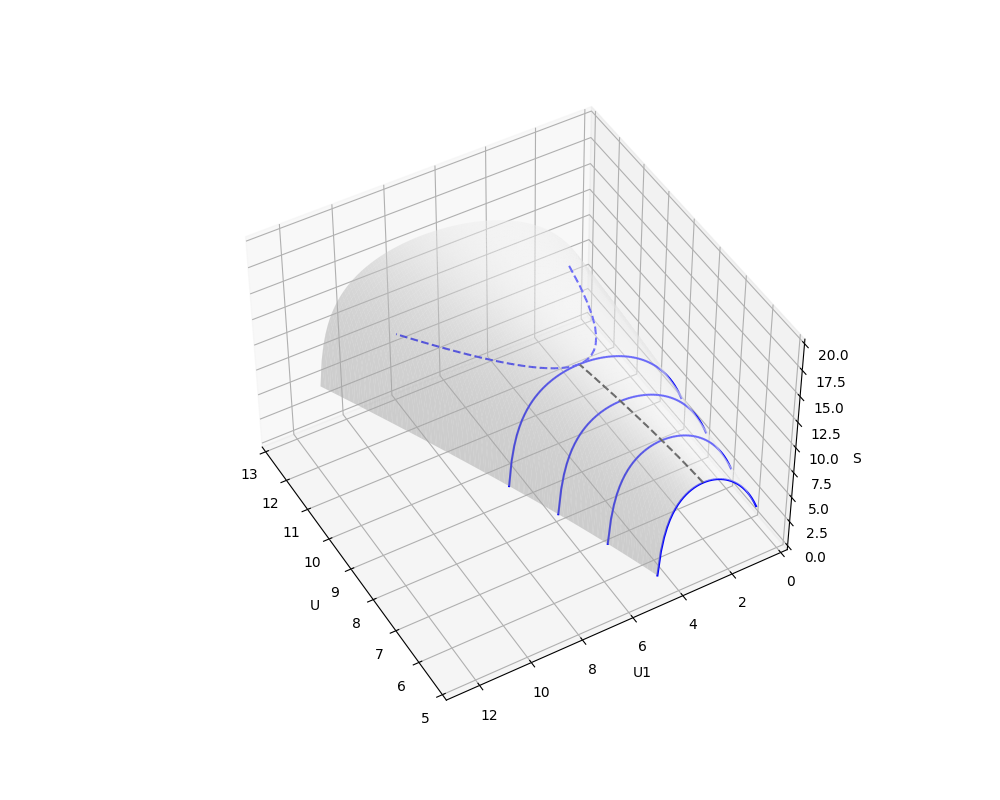
\includegraphics[scale=0.5]{EntropyPlot}
\caption{Plot of an entropy function}
\label{fig:EntropyPlot}
\end{figure}


To be able to work directly with a minimum principle in the energy representation often has advantages. Suppose, for instance, we study systems that are not completely isolated, but permit the exchange of energy with the environment in the form of mechanical work. Then the energy will not be constant, whereas the entropy will be preserved, as no heat flows into the system or out of the system. It is then much more natural to work with a constraint reflecting this, i.e. to consider states with a fixed entropy, and the energy minimum principle then tells us how the system moves through the state space as other constraints are removed.

Finally, we note that of course, as the energy representation and the entropy representation are completely equivalent, both principles hold in both representations, the only difference being that the principle is more easily exploited if the constraint fixes the value of a coordinate and not the value of some function.


\section{The maximal work theorem}

To further illustrate the formalism developed so far and to introduce some terminology that we will need in the sequel let us now consider special types of thermodynamical subsystems. 

A {\em reversible work source} is a subsystem which can change its energy only via changes in its geometry. In other words, it is a system surrounded by impermeable (so that the particle number is constant) and adiabatic (so that no heat transfer is possible) walls. Thus the change of energy for this system is
$$
dU = - P dV = dW
$$
Strictly speaking we would have to phrase this as follows: for every path $\gamma(s)$ in the configuration space that is compatible with the constraints
$$
dU(\gamma(s)) = - P(\gamma(s)) dV(\dot{\gamma(s)})
$$
for all $s$. We will, however, continue to use the simpler notation above if the meaning is obvious. Note that this implies that for any process, the entropy is of this subsystem is actually constant:
$$
dS = \frac{P}{T} dV + \frac{1}{T} dU = \frac{1}{T} (P dV + dU) = 0
$$
Similarly, we can define a {\em reversible heat source} to be a subsystem surrounded by rigid walls, which do however allow heat to pass. Thus, the only energy change that can occur in this subsystem is due to heat transfer, i.e.
$$
dU = T dS = dQ
$$
Thus the change of entropy of such a system is given by
$$
dS = \frac{1}{T} dU = \frac{1}{T} dQ
$$
It is important to note that $T$ in this expression is itself a function of the extensive variables and not necessarily a constant. The {\em heat capacity} of the heat source is defined to be
$$
C(T) = \frac{\partial U}{\partial T}
$$
so that
$$
dQ = C(T) dT
$$
A {\em thermal reservoir} is a reversible heat source with an infinite heat capacity, so that, no matter how large the transfer of heat actually is, the temperature of the reservoir remains constant.

Let us now consider a composite system which is made up of three subsystems, namely a reversible work source, a reversible heat source and a third subsystem, which we call the {\em primary subsystem}, and which is the one which is actually of interest. Let us denote its state by $(U,V,N)$. We assume that the primary subsystem is connected to the reversible work source and the reversible heat source in such a way that it can exchange heat with the heat source and work with the work source.

This is a simple model of an engine that extracts heat from the heat source (which we do not assume to have infinite heat capacity) and transfers a part of the energy received in this way to the work source, for instance by driving some cyclinder. We want to know under which conditions the work delivered to the work source (which we should actually call a work sink in this case) is maximal.

To do this, let us consider the change of energy and entropy that occur during a process. We have seen that the source of work does not undergo any change in entropy, so the total change of entropy is
$$
dS_{tot} = dS + dS_{RHS} = dS + \frac{1}{T_{RHS}} dQ_{RHS} \geq 0
$$
where $S$ is the entropy of the primary system and $S_{RHS}$ is the entropy of the heat source. In particular, we obtain that
$$
dQ_{RHS} \geq - T_{RHS} dS
$$
Now we can use the conservation of energy and the fact that the change in energy for the heat source and work source is entirely due to heat and work by definition to obtain
$$
0 = dU_{tot} = dU + dQ_{RHS} + dW_{RWS}
$$
Thus we find that
$$
dW_{RWS} = - dU - dQ_{RHS} \leq -dU + T_{RHS} dS
$$
with equality if and only if the total entropy does not change at all. A process for which the total entropy is constant is called a {\em reversible process}. Thus we find that the work transferred to the reversible work sink is maximized if the process is reversible. This fact is known as the {\em maximal work theorem}.

Now let us specialize a bit further and assume that the heat source is actually a thermal reservoir, i.e. its temperature is constant. As we assume equilibrium, and as any difference in the temperatures would cause heat to flow further, this implies that in a quasistationary process, the temperature $T$ of the primary subsystem is constant as well and equal to $T_{RHS}$. Then our equations simplify further. In fact, we have
$$
- dQ_{RHS} \leq T dS
$$
and therefore
$$
dW_{RWS} \leq T dS - dU
$$
Now, as the temperature does not change, this is - for this particular type of process - the same as
$$
dW_{RWS} \leq d (TS - U)
$$
Integrating this inequality along a path in the configuration that describes a process subject to the defined constraints, we can conclude that the work that can be delivered by the primary subsystem by drawing heat from a heat reservoir with infinite capacity is bounded by the difference of the function
$$
F = U - TS
$$
between initial and final state. This quantity - which can be defined for any system - is called the {\em Helmholtz free energy} or {\em Helmholtz potential}. We will now see how this potential can be obtained using a Legendre transform.

\section{Legendre transform and free energy}

Let us quickly recall some basic facts about the Legendre transform of a convex function. Assume that we are given a (strictly) convex and (for the sake of simplicity) smooth function
$$
f \colon I \rightarrow \R
$$
defined on some interval $I \subset \R$. The Legendre transform of $f$ is the function $f^*$ given by
$$
f^*(p) = \sup_{x} \{ px - f(x)\}
$$
which is defined for all $p$ for which the supremum exists. As $f$ is supposed to be differentiable, we can maximize this expression by setting the derivative to zero and find that we can alternatively write
$$
f^*(p) = px - f(x)
$$
where $x$ is chosen such that $f'(x) = p$. As we assume that the function is convex and therefore that the second derivative is not zero, the equation
\begin{align}\label{eq:pisfprime}
p = f'(x)
\end{align}
can be solved for $x$ if $p$ is in the range of $f'$, i.e. we can write $x = x(p)$ and express the Legendre transform a bit more precisely as
$$
f^*(p) = px(p) - f(x(p))
$$
as a function on the range of $f'$. Note that the function $x(p)$ does actually depend on the choice of $f$, so care must be taken when using this notation.

Let us now calculate the derivative of the Legendre transform. Applying the product rule and the chain rule, we find that
\begin{align*}
\frac{df^*}{dp} &= \frac{d}{dp} (px(p)) - \frac{d}{dp} f(x(p)) \\
&= p \frac{dx}{dp} + x(p) - f'(x(p)) \frac{dx}{dp} = x
\end{align*}
where we have used equation \ref{eq:pisfprime} in the last line to see that the first and third term cancel. Thus we obtain the fundamental relations
\begin{align*}
p &= \frac{df}{dx} \\
x &= \frac{df^*}{dp}
\end{align*}

\begin{example}
Suppose that we are given functions $f$ and $g$ and know that $g$ is the inverse of $f$. Let us try to express the Legendre transform of $g$ in terms of $f^*$. We now have two functions $x_1(p)$ and $x_2(p)$ given by the relations
\begin{align*}
f'(x_1(p)) &= p \\
g'(x_2(p)) &= p
\end{align*}
Now, as $f$ is the inverse of $g$, we have
$$
g'(f(x_1)) = \frac{1}{f'(x_1)} = \frac{1}{p} = g'(x_2(\frac{1}{p}))
$$
As $g'$ is invertible, we obtain
$$
x_2(\frac{1}{p}) = f(x_1(p))
$$
We therefore find that
\begin{align*}
g^*(\frac{1}{p}) &= \frac{1}{p} x_2(\frac{1}{p}) - g(x_2(\frac{1}{p})) \\
&= \frac{1}{p} f(x_1(p)) - g(x_2(\frac{1}{p})) \\
&= \frac{1}{p}  [ p x_1(p) - f^*(p)  ] - g(f(x_1(p))) \\
&= \frac{1}{p}  [ p x_1(p) - f^*(p)  ] - x_1(p) = - \frac{1}{p} f^*(p)
\end{align*}
or
$$
f^*(p) = - p g^*(\frac{1}{p})
$$
\end{example}

Now assume that we are given a function $f = f(x,y)$ of two variables. We can apply a Legendre transform to one of the two variables, say $x$, while keeping $y$ fixed. Let us call this Legendre transform $f^*$. We then have that
$$
\frac{\partial f^*}{\partial p} = x
$$
and
$$
\frac{\partial f^*}{\partial y} = - \frac{\partial f}{\partial y}
$$
Thus, if we write the total differential of $f$ as
$$
df = p dx + v dy
$$
then
$$
df^* = x dp - v dy
$$
Finally, we remark that the Legendre transform can also be done for a concave function, with the only difference that then,
$$
f^*(p) = \inf_{x} \{ px - f(x)\}
$$

The notation $f^*$ that we have used so far is simple, but not quite adequate for functions of several variables as it does not capture the information to which of the variables we have applied the transform. To rectify this, we follow \cite{Callen}, and, given a function
$$
f = f(x_1, \dots, x_n)
$$
denote the Legende transform with respect to the coordinate $x_i$ as
$$
f[x_i](x_1, \dots, x_{i-1}, p, x_{i+1})
$$


We will now see how this sort of transformation is applied in thermodynamics. Note that in many books, for instance in \cite{Callen}, the term Legendre transform is used for minus one times the Legendre transform as we have introduced it, a convention which we will not adopt.

We have seen that a thermodynamical system is, as long as only macroscopic states in equilibrium are concerned, fully described by the energy as a function of entropy, volume and particle number, i.e. by a relation of the type
$$
U = U(S,V,N)
$$
In some applications, we do have some information on some derived quantities like the temperature. It would then be helpful to be able to express the fundamental relation above in terms of the intensive parameters, i.e. the derivatives of the energy. This is exactly what the Legendre transform is doing.

Consider, for instance, a system for which we have some information on the temperature that we want to utilize. We can then apply the Legendre transform with respect to the entropy to obtain a function of temperature, volume and particle number that - as the Legendre transform can be reversed - contains the same amount of information as the original relation. Note, however, that, by convention, a minus sign is typically inserted at this point. We obtain the quantity
\begin{align}\label{eq:helmholtzenergy}
F(T,V,N) = -U[S] = U - TS
\end{align}
which is exactly the {\em Helmholtz free energy} considered before, but now interpreted as a function of $T$, $V$ and $N$. Thus this is not a pure reorganisation of known quantities, but comes with a change of parameters. If we are given a tuple $(T,V,N)$, we first need to find the entropy $S$ such that 
$$
\frac{\partial U}{\partial S} | (S,V,N) = T
$$
and then use this value to calculate $U$ and $F$. By the general theory developed above, we can also immediately write down an expression for the total 
differential of $F$:
$$
dF = - S dT - PdV + \mu dN
$$
We have already seen above that the Helmholtz energy has an interesting physical interpretation: the maximal work that can be delivered by a system connected to a thermal reservoir is the decrease of the Helmholtz energy. In that sense, the Helmholtz energy is the potential of a system to deliver work at fixed temperature, which explains why this quantity is often called the {\em Helmholtz potential}.

The Helmholtz potential has another important property, which we will now derive. Suppose again that we are considering a system which is in contact with a thermal reservoir of temperature $T$. Consider some process which is quasi-static and in particular keeps the temperature of our system constant and equal to the temperature of the reservoir. Differentiating equation \ref{eq:helmholtzenergy}, interpreted as defining a function of $(U,V,N)$, and restricting to tangent vectors along the hypersurfaces of constant temperature so that $dT = 0$, we obtain
$$
dF = - P dV + \mu dN
$$
Now consider the total entropy of the composite system that consists of the system of interest and the thermal reservoir. As the volume and particle number of the thermal reservoir are constant, we can calculate the 
total differential of the entropy of the reservoir and obtain
$$
d S_R = \frac{1}{T} dU_R = - \frac{1}{T} dU + \frac{1}{T} dU_{tot}
$$
so that the differential of the total entropy is
\begin{align*}
d S_{tot} &= dS - \frac{1}{T} dU + \frac{1}{T} dU_{tot} \\
& = \frac{1}{T} (P dV - \mu dN) + \frac{1}{T} dU_{tot} \\ 
&= - \frac{1}{T} dF + \frac{1}{T} dU_{tot}
\end{align*}
or
$$
T dS_{tot} = - dF + dU_{tot}
$$
Let us now suppose that we let the composite system somehow interact with the environment. If this interaction is reversible, so that the total entropy of the system $S_{tot}$ is constant, the left hand side of this equation is zero. This implies that a state minimizes the total energy if and only it is minimizes the Helmholtz potential of the primary subsystem. Thus the results from section \ref{sec:minimalinternalenergy} immediately yield a minimum principle for the Helmholtz energy: {\em the equilibrium state of a system which is in diathermal contact with a thermal reservoir minimizes the Helmholtz potential}. Note that the same conclusion holds if the energy of the overall system is conversed. Then $dF = - T dS_{tot}$ so that the Helmholtz free energy is minimized if and only if the total entropy is maximized.


Obviously we can apply Legendre transforms to the other extensive variables as well and to combinations of them. Functions obtained in this way are called {\em thermodynamic potentials}. We will not got into further details in this short introduction, but only mention the enthalpy, which is the Legendre transform with respect to the volume, and the Gibbs free energy, which is the Legendre transform with respect to volume and entropy at the same time and given by
$$
G(T, P, N) = U - TS + PV
$$
These potentials have properties similar to the Helmholtz energy, for instance we can deduce in a similar way that the Gibbs free energy is minimized in equilibrium if a process is constrained to a fixed temperature and pressure - we will actually demonstrate an application of this in the next section.



As an example, let us calculate the Gibbs energy of an ideal gas. In a previous section, we have already derived the following expression for the chemical potential.
$$
\mu  = -T s_0 - T R \ln \big[ \big( \frac{U}{U_0} \big)^c \frac{V}{V_0} N^{-c - 1}  \big] + (c+1) RT 
$$
Let us express the chemical potential in terms of temperature and pressure instead of energy and volume. Using the ideal gas laws, we easily obtain
$$
\big( \frac{U}{U_0} \big)^c \frac{V}{V_0} N^{-c - 1} = N_0^{-c - 1} \big( \frac{T}{T_0} \big)^{c+1} \frac{P_0}{P}
$$
where $N_0$ is the particle number of our reference state. When we conveniently choose this to be $N_A$, so that our reference state contains one mole of substance, we therefore find that
$$
\mu  = -T s_0 - T R \ln \big[ N_A^{-c - 1} \big( \frac{T}{T_0} \big)^{c+1} \frac{P_0}{P}  \big] + (c+1) RT
$$
showing that {\em the chemical potential of an ideal gas in isolation does not depend on the particle number}. Based on the results in the appendix on homogenous functions, this is what we expect, as the chemical potential is homogenous of degree $0$ in $N$ and therefore constant (along rays, but as there is only one particle involved this implies that is does not depend on $N$). This only becomes apparent if we express the chemical potential really in terms of $T$, $P$ and $N$ alone and unravel all hidden dependencies on $N$, for instance in $S$.  As the Gibbs energy is homogenous in $N$,  the Gibbs energy of a system with $N$ particles is simply $\mu N$. Spelling this out explicitly and collecting terms, we find that
$$
G(T, P, N) = \frac{N}{N_A} \frac{T}{T_0} G_0 - N T R  \ln \big[ \big( \frac{T}{T_0} \big)^{c+1} \frac{P_0}{P}  \big]
$$
where $G_0$ is the Gibbs energy of one mole of our gas at standard conditions.

\section{The Carnot cycle and heat engines}

We have already briefly discussed heat engines and demonstrated that the second law of thermodynamics (in combination with the first law) implies that there is an upper bound on the efficiency of a heat engine. In fact, we have seen that for a heat engine in contact with a heat bath of temperature $T_h$ and a second heat bath of temperature $T_l < T_h$, the efficiency with which the engine can turn heat drawn out of the hotter heat bath into work is at most
$$
1 - \frac{T_l}{T_h}
$$
We note that the pure fact that there is a bound is not too surprising - by the conservation of energy, the efficiency cannot exceed one. The more interesting part is that the bound is lower than one. In fact, the second law tells us that whenever we let heat flow between two bodies with different temperatures, there is a price we have to pay - an increase in entropy - and this limits the efficiency of a heat engine in addition to the limit given by the conservation of energy.

Let us now try to understand how a process that actually achieves this bound could look like. Thus we need to devise a cycle that our system undergoes and which takes it back to its original state while drawing heat out of the hot reservoir with temperature $T_h$, converting it into work and then letting excess heat flow into the cold reservoir with temperature $T_l$. 

The first observation that we can make is that in order to avoid any unnecessary loss of entropy, our process needs to be quasi-static, and for any transfer of heat, the difference in temperature between the involved bodies should be as small as possible. So imagine we start with a state I in which our system has a temperature which is only a tiny bit smaller than $T_h$, i.e. $T \approx T_h$. Then a certain amount of heat $Q_h > 0$ will flow from the hot reservoir into the engine. During this time, the entropy of the engine changes by an amount
$$
\Delta S_A = \frac{Q_h}{T_h}
$$
Now we want to keep the temperature of our engine constant while the heat flows, which usually means that we have to let the engine do some work by expanding until it reaches a certain state $II$. Next, we let the engine undergo an adiabatic expansion. During this adiabatic expansion, the engine will do some additional work on the environment and its temperature will drop again. However, as no heat flows, the entropy will not change during that part of the cycle. We let the engine expand until its temperature has reached a value slightly above $T_l$. Denote this state by  $III$. 

In the third part of the cycle, we let the machine undergo another isothermal process during which it transfers some heat $Q_l < 0$ into the cold reservoir. Again, this will trigger a change in entropy given by 
$$
\Delta S_C = \frac{Q_l}{T_l}
$$
Finally, we let the engine decrease its volume further in an adiabatic process during which it consumes some work from the environment. Thus the total change in entropy is 
$$
\Delta S_A + \Delta S_C
$$
However, the entropy is a state variable and our process is a cycle, so that the total change in entropy is zero. Thus
$$
\Delta S_A  = -  \Delta S_C
$$
or 
$$
\frac{Q_h}{T_h} = - \frac{Q_l}{T_l}
$$
so that
$$
\frac{T_l}{T_h} = - \frac{Q_l}{Q_h}
$$
Similarly, the total change in energy is zero. By the first law, this implies that
$$
0 = Q_h + Q_l + W
$$
where $W$ is the total work done by the environment. Thus
\begin{align*}
W &= - Q_h - Q_l  \\
&= - Q_h (1 + \frac{Q_l}{Q_h}) \\
&= - Q_h  (1 - \frac{T_l}{T_h})
\end{align*}
We therefore find that
$$
\frac{-W}{Q_h} = 1 - \frac{T_l}{T_h}
$$
Now $W$ is the work done on the system, so that $-W$ is the work that is done on the environment. The left hand side is therefore exactly the efficiency as we have defined it earlier, and we find that the efficiency of a Carnot engine is in fact equal to the theoretical limit. 

\begin{figure}[h]
	\centering
	\begin{tikzpicture}
		% axes
		\draw[->] 
		(-.5, 0) -- (-.5, 5) node[left=.1cm] {P};
		\draw[->] 
		(-.5, 0) -- (5.5, 0) node[below=.1cm] {V};
		% arcs
		\draw[-] (3.12,2.52) arc (259:230:6.3);
		\draw[-] (3.12,2.52) arc (220:240:5);
		\draw[-] (4.45,1.38) arc (260:230:6);
		\draw[-] (1.67,2.68) arc (265:193:1.6);
		% labels
		\node[label=I]  at (0.4,3.8) {};
		\node[label=II]  at (3.2,2.6) {};
		\node[label=III]  at (4.5,1.4) {};
		\node[label=IV]  at (1.6,1.9) {};
		% text
		\node at (1.8,3.6) {\tiny isothermic at $T_h$};
		\node at (4.1,2.3) {\tiny adiabatic};
		\node at (2.5,1.4) {\tiny isothermic at $T_l$};
		\node at (.6,2.6) {\tiny adiabatic};
	\end{tikzpicture}
	\caption{Carnot cycle in V-P space}\label{fig:carnotpv}
\end{figure}

To visualize the process, it is useful to display the process as a curve in our configuration space. The first diagram (\ref{fig:carnotpv}) displays this process in the state space spanned by pressure $P$ and volume $V$. We start at state $I$ with an isothermic expansion at temperature $T_h$, then switch at some point to an adiabatic expansion, followed by an isothermal compression at temperature $T_l$ and finally use an adiabatic process to return to our starting point. 

\begin{figure}[h]
	\centering
	\begin{tikzpicture}
		% axes
		\draw[->] 
		(-.5, 0) -- (-.5, 5) node[left=.1cm] {T};
		\draw[->] 
		(-.5, 0) -- (5.5, 0) node[below=.1cm] {S};
		% arcs
		\draw[-] (1, 4) -- (4, 4);
		\draw[-] (4, 4) -- (4, 1);
		\draw[-] (4, 1) -- (1, 1);
		\draw[-] (1, 1) -- (1, 4);						
		% labels
		\node[label=I]  at (0.7,4) {};
		\node[label=II]  at (4.2, 4) {};
		\node[label=III]  at (4.2,.2) {};
		\node[label=IV]  at (.7,.2) {};
		% text
		\node at (2.4,4.2) {\tiny isothermic at $T_h$};
		\node at (4.7,2.5) {\tiny adiabatic};
		\node at (2.4,.8) {\tiny isothermic at $T_l$};
		\node at (.3,2.5) {\tiny adiabatic};
	\end{tikzpicture}
	\caption{Carnot cycle in S-T space}\label{fig:carnotst}
\end{figure}


If we describe the process in terms of the conjugated variables $S$ and $T$, we obtain diagram \ref{fig:carnotst}. Here we see that during the first and third phase of the process, the temperature remains constant, while the entropy changes, as heat is transferred in an isothermal process. In phase two and four, no heat is transferred, and as we assume the process to be quasi-static, the entropy does not change. Again, the cycle returns to its original state as $S$ and $T$ are state variables.

Also note that the Carnot cycle demonstrates nicely that the amount of heat emitted or absorbed is actually path-dependent. In diagram \ref{fig:carnotpv}, the system can move from state I to state III by either following the first part of the cycle or the (reversed) second part of the cycle. In the first case, the amount of heat absorbed is $Q_h$, in the second case, this is $Q_l$, and our calculation shows that these are not equal unless $T_h = T_l$.

\section{The van der Waals model}

In this section, we put the principles discussed so far into action, using the van der Waals model to describe an actual gas. In contrast to an ideal gas, that ignores interactions between the particles, the van der Waals model describes a substance with interaction. In this model, the fundamental equation is
$$
F = F(T,N,V) = - N k_B T [   \ln(\frac{V-bN}{N}) + \frac{3}{2} \ln (k_B T)] - a \frac{N^2}{V}
$$
where $a$ and $b$ are positive constants that account for interactions between the particles ($a$) and the volume of the particles ($b$). As $F$ is minus the Legendre transform of $U=U(S,V,N)$, we know that
$$
S = - \frac{\partial F}{\partial T} = \frac{3}{2} N k_B + 
N k_B [\ln \frac{V-bN}{N} + \frac{3}{2} \ln k_B T]
$$
Using the relation
$$
U = TS + F
$$
we can therefore find an expression for $U$ as
$$
U(T,N,V) = \frac{3}{2} N k_B T - a \frac{N^2}{V}
$$
We can also calculate the pressure and the chemical potential easily in this representation. For instance, the pressure is given by 
$$
P = - \frac{\partial F}{\partial V} =  \frac{N k_B T}{V-bN}  - a \frac{N^2}{V^2}
$$
which yields an expression for the Gibbs free energy
$$
G = F + PV = - N k_B T [ \ln\frac{V-bN}{N} + \frac{3}{2} \ln k_B T] + \frac{N k_B TV}{V-bN} 
-\frac{2aN^2}{V	}
$$

Let us look at some quantities that are typically used to describe the behavior of our system. Then first quantity is called the {\em isothermal compressibility}. It measures to what extent a gas or fluid can be compressed when some pressure is exercised, and is defined as
$$
\kappa_T = - \frac{1}{V}  (\frac{\partial V}{\partial P})_{T,N}
$$
Here we use the usual notation that the variables that are to be fixed are added as a subscript to the partial derivative. So we need to express $V$ in terms of $P,T$ and $N$ and then take the partial derivative with respect to $P$. Clearly, the inverse of this quantity is
$$
\frac{1}{\kappa_t} = - V  (\frac{\partial P}{\partial V})_{T,N}
$$
That can easily be computed. We have
$$
(\frac{\partial P}{\partial V})_{T,N} = - \frac{N k_B T}{(V - bN)^2} + \frac{2aN^2}{V^3}
$$
For $a = 0$, corresponding to the case of an ideal gas, this is clearly negative. This corresponds to a positive value of the compressibility and is what we would expect - when we increase the pressure, the volume will decrease. However, for positive $a$, this derivative can have zeros. This can be a simple zero, or a zero of higher order. The point $(T_c, V_c)$ where a multiple zero occurs, i.e. for which
$$
(\frac{\partial P}{\partial V})_{T,N}  = 0
$$
and
$$
(\frac{\partial^2 P}{\partial V^2})_{T,N}  = 0
$$
is called the {\em critical point}. This corresponds to the equations
\begin{align*}
\frac{N k_b T}{(V-bN)^2} &= \frac{2aN^2}{V^3} \\
\frac{N k_b T}{(V-bN)^3} &= \frac{3aN^2}{V^4} 
\end{align*}
Dividing the first by the second condition yields
$$
V - bN = \frac{2}{3} V
$$
so that 
$$
V_c = 3 b N
$$
Plugging this into the first equation gives
$$
k_B T_c =  \frac{8a}{27b}
$$
The pressure at the critical point is then easily calculated to be
$$
P_c = \frac{a}{27b^2}
$$
It is useful and simplifies a few calculations to express the temperature and pressure in a dimensionless way relative to the critical point. Thus we introduce the notation
\begin{align*}
\bar{T} = \frac{T}{T_c} \\
\bar{V} = \frac{V}{V_c} \\
\bar{P} = \frac{P	}{P_c} 
\end{align*}
Then, for instance, the expression for the normalized pressure becomes
$$
\bar{P} = \frac{8 \bar{T}}{3 \bar{V}-1} - \frac{3}{\bar{V}^2}
$$
(see \cite{Callen}, example 1 in section 9.4 for a reassuring cross-check).
We also see that to solve this for the volume given temperature and pressure, we have to find the roots of a third-order polynomial in the volume. Thus there will in general be three roots. We will soon see that one of these roots is in the instable region, while the other two correspond to the volumes of the gas and liquid phase.


In figure \ref{fig:VanDerWaals}, we have displayed some of the relations between pressure, temperature and volume. 


\begin{figure}[ht]
\centering
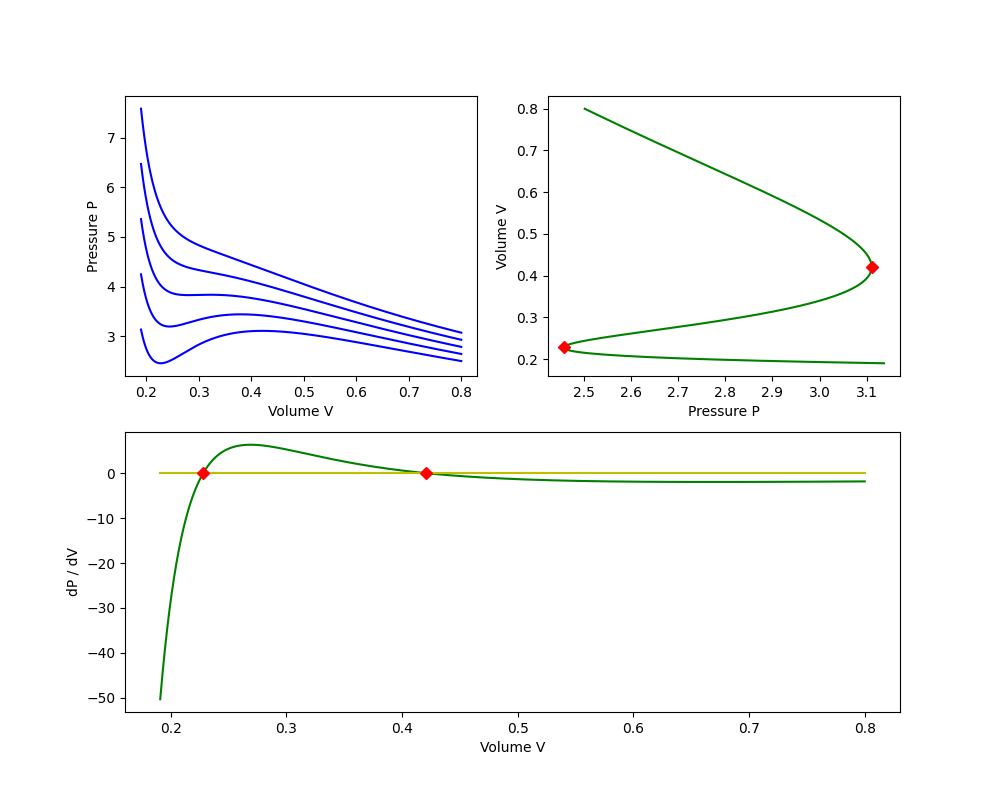
\includegraphics[scale=.5]{VanDerWaals}
\caption{P-V diagrams for a Van der Waals fluid (a=1.05, N=1, b=0.1, k=1)}
\label{fig:VanDerWaals}
\end{figure}

The diagram on the left displays the dependency of $P$ on $V$ for four different values of $T$ between 2.9 (lowest line) and 3.3 (highest line). The second line from the top has $T = T_c$. We clearly see that the nature of the lines changes as expected and we introduce zeros of the derivative, i.e. extremal points. 

An example for such a curve (for $T=2.9 = 0.93 T_c$) is displayed in detail in the picture at the right, this time with the axis reverted. We see that, as we expect, the relation between $V$ and $P$ can no longer be inverted, i.e. for one value of $P$, there is more than one matching value of $V$. The zeros of the derivative are marked with red diamonds. The same markers have been added in the diagram at the bottom, which displays the partial derivative
$$
\frac{\partial{P}}{\partial V}
$$	
for $T=2.9$ and $N=1$. In the area between these points (that correspond to an infinitely large value for the isothermal compressibility), the derivative is positive. This means that exercising pressure would in fact cause the material to expand, which is clearly unphysical and would lead to an unstable behavior  (if we place this material in a small container, an expansion would in turn increase the pressure exercised by the air in the container and the process would, once initiated, continue). Thus there is a {\em region of the phase space that does not represent stable systems}. Intuitively, when the state moves along the isothermal, it will proceed directly from a point on the right of the instable region to a point on the left of the region, with a discontinuous behavior of the volume. This is an indication of a {\em phase transition}.

This might sound a bit strange, but recall that all the quantities that we are dealing with are only defined in equilibrium, and we have essentially argued that certain regions of the phase space do not allow for an equilibrium. Thus when a system reaches this region, it will no longer be able to maintain an equilibrium. It will continue to evolve its microstate, and at some point, when the phase transition is complete, it will reappear in the configuration space, in alignment with our previous discussion of quasi-static processes. Thus it is not the system that somehow evolves in an unpredictable way during a phase transition, it is our description in terms of equilibria that breaks down at this point.

Let us take a closer look at the role that the Gibbs energy plays in a phase transition. For that purpose, let us assume that a portion of the gas described by the van der Waals equations is contained in a vessel and let us consider a system that consists of a comparatively small, but fixed number of particles within the vessel, but can change its volume and its internal energy - this could just be a small bubble within the system that can absorb or emit heat and shrink or grow. 

We can then model the part of the vessel outside this small subsystem as a heat reservoir that keeps the temperature $T$ stable and, at the same time, as a pressure reservoir, so that the pressure $P$ is constant as well. The subsystem itself could again be a composite system and therefore be described by its total energy, volume and other, internal parameters. If we use the index R to indicate that a quantity refers to the reservoir and quantity without subscript to refer to our small subsystem, we then have
\begin{align*}
dU_{tot} &= dU + dU_R  \\
&= dU - P dV_R + T dS_R \\
&= dU + P dV - T dS + T dS_{tot} \\
&= dU + d(PV) - d(TS) + TdS_{tot} = dG + TdS_{tot}
\end{align*}
where we have used that the number of particles within the subsystem and therefore within the reservoir is constant to get from the first line to the second line, the fact that the total volume is constant to get from there to the third line and the fact that temperature and pressure are constant in the last line.

When we now assume in addition that the total energy is preserved and therefore $dU_{tot} = 0$ (this even holds if the total energy is not preserved but merely minimized), we find that 
$$
dG = - T dS_{tot}
$$
As the total entropy has a maximum in the equilibrium state, we can conclude that the Gibbs energy has a minimum in the equilibrium state. More general, for systems that are in touch with a heat and a pressure reservoir, the Gibbs energy is minimized by the equilibrium state subject to the condition of constant total entropy - this is the equivalent of the respective condition for the Helmholtz energy if merely the temperature is kept stable by a heat reservoir.

Armed with this information, let us now get back to the van der Waals equation and study in more detail the phase transition along an isotherm. For that purpose, we want to express the Gibbs energy in terms of the normalized variables used earlier. We are only interested in the terms depending on the volume $\bar{V}$, and we will use the normalized molar Gibbs energy, i.e.
$$
g = \frac{G}{N k_B T_c}
$$
The first term that depends on $V$ can be written as follows
\begin{align*}
- \frac{1}{N k_B T_c} N k_B T  \ln\frac{V-bN}{N}  &= - \frac{T}{T_c}  \ln\frac{V-bN}{N} \\
&= - \bar{T} \ln\frac{3 \bar{V} b N - bN}{N} \\
&= - \bar{T} \ln b (3 \bar{V}   - 1) = - \bar{T} \ln  (3 \bar{V}   - 1) - \bar{T} \ln b
\end{align*}
where we have used the relation
$$
V = V_c \bar{V} = 3 \bar{V} b N
$$
We will only keep the first logarithm and move the second term into the part that does not depend on $V$. Similary, the second term in the Gibbs energy turns into
\begin{align*}
\frac{1}{N k_B T_c}	\frac{N k_B TV}{V-bN} &= \bar{T} \frac{V}{V - bN} \\
&= \bar{T} \frac{3 \bar{V} b N}{3 \bar{V} b N - bN} \\
&= \bar{T} \frac{3 \bar{V} }{3 \bar{V} - 1} \\
&= \bar{T} \frac{3 \bar{V} - 1 }{3 \bar{V} - 1} + \bar{T} \frac{1 }{3 \bar{V} - 1} = \bar{T}  + \bar{T} \frac{1 }{3 \bar{V} - 1}
\end{align*}	
Again, we move the first term into the part of the Gibbs energy that only depends on the temperature. Finally, the third term of the Gibbs energy that depends on $V$ turns into
\begin{align*}
- \frac{1}{N k_B T_c} \frac{2aN^2}{V} &= - \frac{1}{k_B T_c} \frac{2aN}{3 b N \bar{V}} \\
&= - \frac{27b}{8a} \frac{2a}{3 b \bar{V}} = - \frac{9}{4 \bar{V}}
\end{align*}
where we have used that $k_B T_c =  \frac{8a}{27b}$. 
Collecting all terms depending on $V$, we thus arrive at
$$
g =  - \bar{T} \ln (3\bar{V} - 1) 
+  \frac{\bar{T}}{3\bar{V} - 1} - \frac{9}{4 \bar{V}} + f(\bar{T})
$$
with a function depending on $\bar{T}	$ only (usually one would write down the Gibbs energy in terms of temperature and pressure, but in this case, we cannot do this as the volume is not a function of pressure as it is the case in the absence of phase transitions). The part depending on $V$ and the corresponding P-V curve for a fixed temperature $T = 0.85*T_c$ are plotted in figure \ref{fig:VanDerWaalsMaxwell}.

\begin{figure}[ht]
\centering
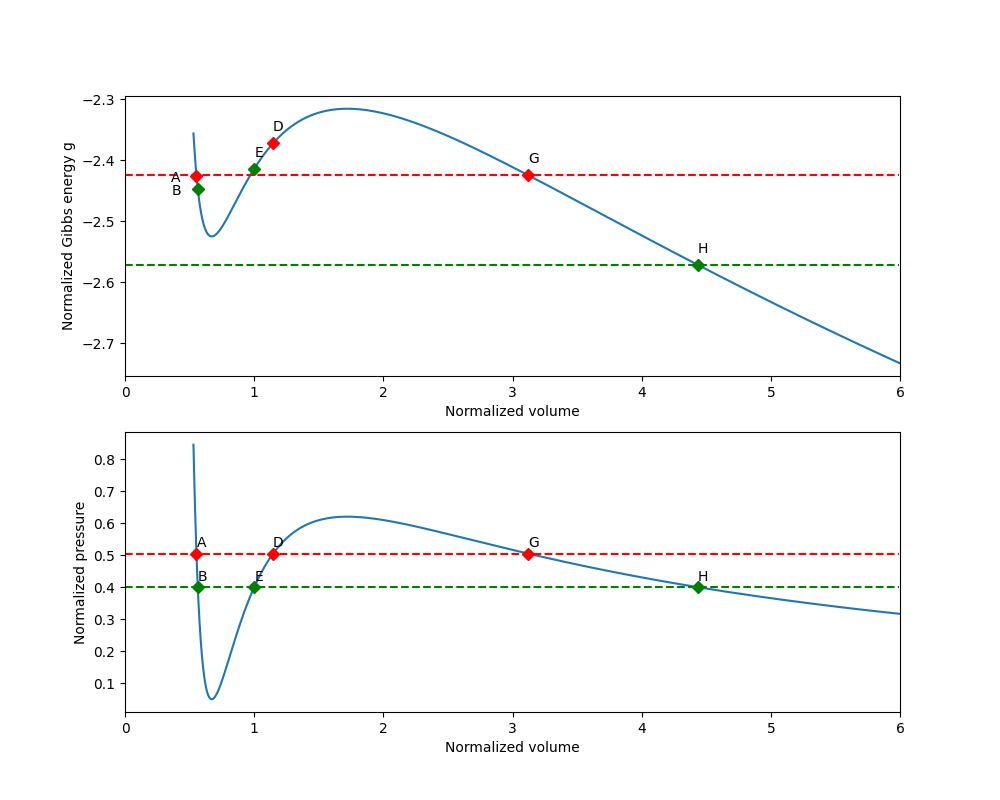
\includegraphics[scale=0.5]{VanDerWaalsMaxwell}
\caption{Gibbs energy along a van der Waals isotherm}
\label{fig:VanDerWaalsMaxwell}
\end{figure}

When a state moves along the isotherm starting below $H$, it will, at some point, experience a phase transition. It will then disappear from the configuration space and appear again at the left hand side of the diagram. It could do so at point H and reappear at point 
B (which, as we can see in the lower diagram, are two points with the same pressure but different values) or it could transition into the second phase upon reaching point G and reappear at point A (another pair of points with the same pressure and different volumes). How can we determine at which point the transition really happens?

To understand this, consider a little subsystem as before, for which we now know that the Gibbs energy has a minimum, but this time suppose that this system is by itself a composition of two subsystems, which are both in contact with the surrounding reservoirs. The first subsystem, with $N_1$ particles and volume $V_1$, is still in the phase I on the left hand side of the unstable region, whereas the second subsystem, with $N_2$ particles and occupying volume $V_2$, is already in phase II. In each of the phases, the Gibbs energy it proportional to $g(T, V_i) N_i$ with $g$ as above. As the Gibbs energy is additive in the particle number (and pressure and temperature are the same for both subsystems), we know that
$$
G = g(T, V_1) N_1 + g(T, V_2) N_2 = g(T, V_1) N_1 + g(T, V_2) (N - N_1)
$$
where $N$ is the number of particles in our subsystems. Now this is a minimum if and only if
$$	
0 = \frac{G}{\partial N_1} = g(T, V_1) - g(T, V_2)
$$
i.e. if the Gibbs energies at both sides of the instable region are identical. If the Gibbs energies are different, say if $g(T, V_1) > g(T, V_2)$, then the system is not stable as transferring additional substance from phase I to phase II will increase the Gibbs energy. Thus we can conclude that we can have a stable state if and only if the two Gibbs energies are equal.

Assuming stability, let us now take a look at the plot of the Gibbs energy. We see that for the pair of states H and B, the Gibbs energy on the left hand side of the unstable region is much higher than the energy on the right hand side. As the system is striving for a minimum of the Gibbs energy, no transition from H to B will take place. If, however, we increase the pressure further and the state moves further along the isotherm and eventually reaches G, the Gibbs energies on both sides (points G and A) will be equal. So at this point the transition will take place. We note that this will make the Gibbs function continuous as a function of the pressure $p$. 

Put differently, the points G and A mark two states in two different phases with the same pressure and temperatures, but different volumes and hence densities, that have the same Gibbs free energy and are therefore able to coexist in a stable state. This is called a {\em coexistence state}. If we think of the two phases as gas and liquid phase, this is just the boiling point. Thus, there is one pressure for which coexistence is possible for each given value of the temperature less than $T_c$. When plotted into a P-T diagram, as in figure \ref{fig:VanDerWaalsPhaseDiagram} (where we have again plotted the normalized pressure and temperature), we find a curve that ends at the critical point. A diagram like this is called a {\em phase diagram}.

\begin{figure}[ht]
\centering
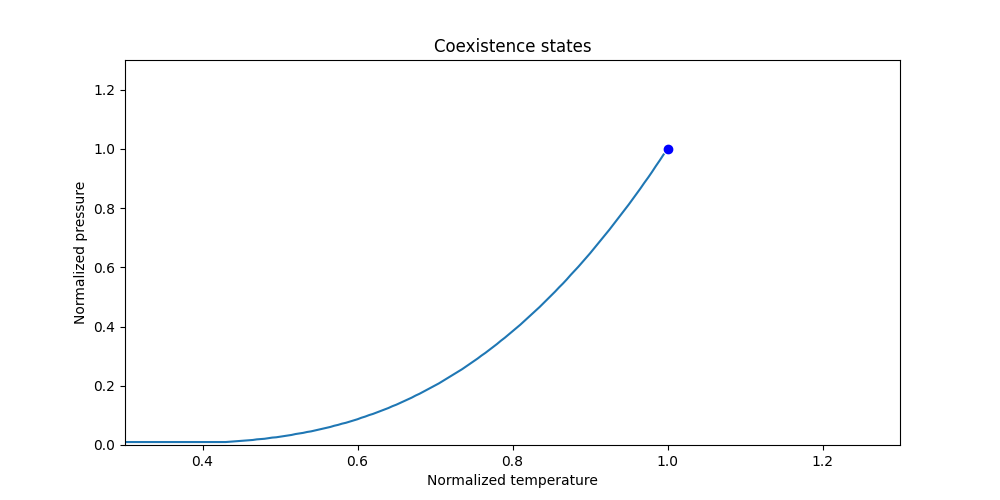
\includegraphics[scale=0.5]{VanDerWaalsPhaseDiagram}
\caption{Phase diagram for a van der Waals system}
\label{fig:VanDerWaalsPhaseDiagram}
\end{figure}
 
 	
\section{More on phase transitions}
 
Some textbooks take a different approach to phase transitions that is based on the properties of the Helmholtz free energy. As a few important details are typically left out when this is presented, it might be worth to take a closer look at this argument. We will again use the van der Waals gas as an example, but the structure of the argument does not depend on any specifics of this system. 


To simplify some of the calculations, let us íntroduce a normalized Helmholtz energy
$$
f = \frac{F}{k_B N T_c}
$$
as we have done it for the Gibbs free energy and find an expression for it in terms of the reduced quantities. Reusing some of the calculations that we have done for the normalized Gibbs energy, we find that
$$
f =  - \bar{T} \ln (3\bar{V} - 1) - \frac{9}{8 \bar{V}} + f_0(T)
$$
with a function $f_0$ depending on the temperature alone. To get an idea for the shape of this curve, let us take a look at diagram \ref{fig:VanDerWaalsHelmholtz}

\begin{figure}[ht]
	\centering
	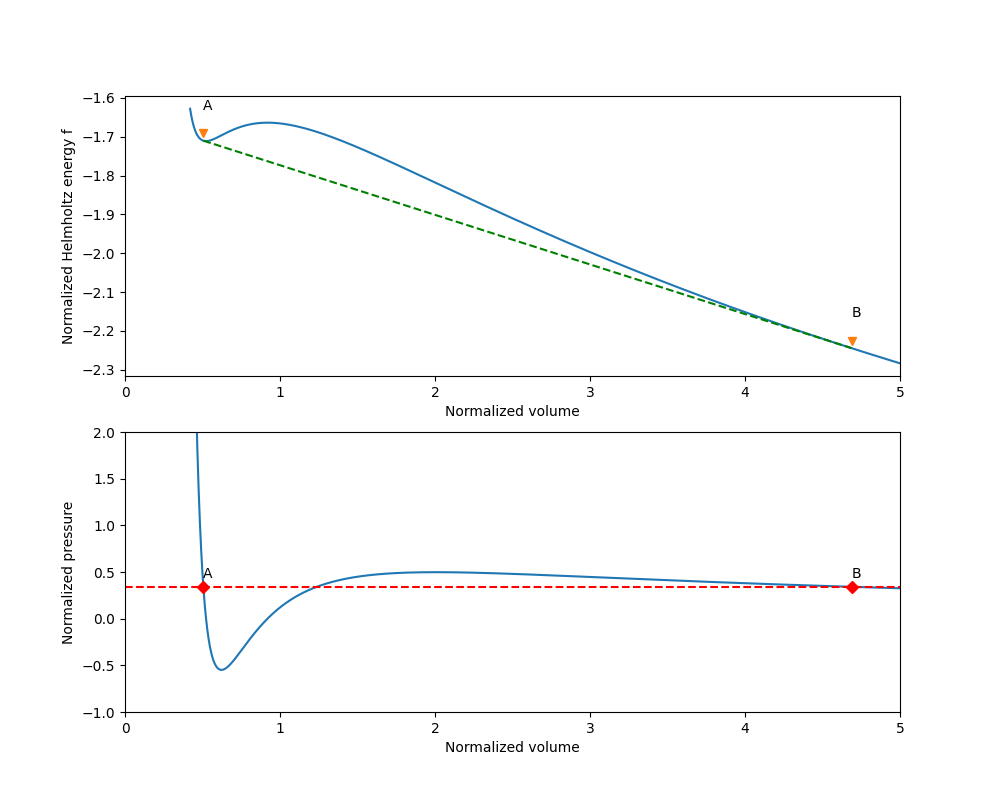
\includegraphics[scale=0.5]{VanDerWaalsHelmholtz}
	\caption{Helmholtz energy of a van der Waals gas}
	\label{fig:VanDerWaalsHelmholtz}
\end{figure}


The upper part of this diagram displays the free Helmholtz energy as a function of the reduced volume while the lower part of the diagram shows the corresponding values of the reduced pressure which (up to a constant due to normalization) is the derivative of the Helmholtz energy. We already know that we will find two volumes $V_A$ and $V_B$ for which the pressure is the same, which we can interpret as the volumes of the liquid phase and the gas phase exposed to the same pressure. 

We also know that the pressure is - up to a normalization factor that is due to our usage of reduced quantities - minus the derivative of the Helmholtz energy with respect to the reduced volume. In addition, the derivative of the pressure with respect to the volume changes its sign and is positive in a small region. In this region, the second derivative of the Helmholtz energy is negative, meaning that the Helmholtz energy fails to be a convex function of the volume in this range.

Let us try to understand what this means. Suppose we are looking at a temperature between $V_A$ and $V_B$. 

\section{The microcanonical ensemble}

Up to now, we have taken the existence of the entropy for granted respectively formulated it as a postulate, and focused our attention on macroscopic states and their development over time. We will now explore microstates and find that the entropy can in fact be defined as a statistical quantity. 

To describe microstates, let us consider a system with a finite state space (we consider discrete state spaces for the sake of simplicity, but for most of what follows, the generalization to a continuous state space is obvious). Thus we have a set
${\mathcal S}$ of states and assume that each of the states describes the system completely from a microscopical point of view. We also assume that each microstate has a well defined total energy $E$, i.e. that we have an energy function 
$$
E \colon {\mathcal S} \rightarrow \R
$$
Note that other macroscopic quantities like the temperature and the pressure are only defined in equilibrium, so we should not expect them to be given by a function on the state space - we will get back to this point later.

The state space can be very general, and it is useful to introduce some examples that illustrate the concepts that we will discuss.

\begin{example}[The two state system]
Let us assume that we have a substance which is composed of particles that only have two possible discrete states. One of these states has energy 0, the other state has energy $\epsilon$. If we consider a system of $N$ such particles, then we can describe the microstate of the system by specifying, for each particle, whether it is in the ground state or in the excited state. Thus we can represent each state as a vector in $\{0,1\}^N$ and therefore the state space has $2^N$ elements. The energy function is given by
$$
E(x_1, x_2, \dots, x_n) = \epsilon\sum_i x_i
$$
An example could be a paramagnetic substance in a magnetic field which we model as being composed of microscopic dipoles and the state reflects the orientation of the dipole relative to an external magnetic field (parallel or antiparallel).
\end{example}

\begin{example}[The Einstein solid]
Let us now consider a very simple model for a solid, developed by A. Einstein. We consider a collection of $N$ very small microscopic systems, for instance particles in a crystalline solid that we envision as being bound to a specific equilibrium location by a harmonic force. That is, each particle is an independent system described by a harmonic oscillator (so the model ignores interactions between the particles) in three dimensions, or, equivalently, by three harmonic oscillators in one dimension. Thus the entire system consists of $3N$ independent harmonic oscillators. We assume that for each oscillator, the energy levels are given by $n \hbar \omega$ with the same $\omega$ for all oscillators. We therefore can describe each oscillator by its occupation number $n$, and consequently the state space is given by ${\N}^{3N}$, and the energy of a microstate is given by
$$
E(n_1, n_2, \dots, ) = \hbar \omega \sum_i n_i
$$
\end{example}

Let us now again consider some system, described by a state space ${\mathcal S}$ and macroscopic variables, say $U, V, N$ and maybe some other variables $\{X_i \}$. We seek to relate the entropy of the system to the microstates. Obviously, different microstates will give us different values for the energy. In the example of the Einstein model, we expect that the total energy will be equal to the sum of the energies of all oscillators and therefore depend on the state. There will, however, be some subset of the state space that is compatible with the macrostate. The number of microstates that are compatible with a given macrostate is called the {\em multiplicity} of the microstate and is conventially denoted as
$$
\Omega(U,V,N, \{ X_i\})
$$
even though this collides a bit with the usual usage of $\Omega$ in probability theory and statistics (this is the reason why we use the letter ${\mathcal S}$ for the state space).

If a system is composed of two subsystems, then there will be a number of compatible microstates for the first system and a number of compatible microstates for the second system, and if we assume the systems to be initially isolated, the total multiplicity is
$$
\Omega = \Omega_1 \Omega_2
$$
Now let us suppose that we remove a barrier between the systems, and allow some particles to pass from one system to the other system or allow the particles in the two systems to interact. As we have removed a constraint, it is reasonable to assume that the number of microstates which are compatible with the remaining constraints will increase. Thus we now have
$$
\Omega \geq \Omega_1 \Omega_2
$$
Thus we have found a quantity which is multiplicative with respect to subsystems and tends to increase as constraints are removed. This is already very similar to the entropy, with the difference that the entropy is additive, not multiplicative. This can be fixed with a logarithm, and we arrive at the following definition which goes back to S. Boltzmann.

\begin{defn}
The {\em Boltzmann entropy} of a system with a given macrostate $(U,V,N, \{X_i\})$ is the logarithm of the number of microstates compatible with the values of the macroscopic variables, i.e.
$$
S(U,V,{\ X_i}) = k_B \ln \Omega(U,V,\{ X_i\})
$$
The constant $k_B$ is called the {\em Boltzmann constant}.
\end{defn}

There is a little subtlety concerning this definition that is worth mentioning. In many cases, we will want to apply this to system of many particles which have discrete energy levels. The actual energy of a system is then the sum of the individual energies and can therefore also take only discrete values. Thus $\Omega(U)$ would be zero for almost all values of $U$ and the entropy would be minus infinity. To avoid this, Callen proposes in \cite{Callen} section 15.5 that we technically have to consider all states with energies in a range $(U - \Delta U, U + \Delta U)$ and makes a nice argument why for a sufficiently high-dimensional state space, the choice of $\Delta U$ does not matter. However, this creates a certain conflict with the idea that the entropy is a function of the macroscopic variables and thus depends on the average energy of a system, not on the exact value of the energy in a certain state. This can be resolved by thinking of both, the entropy and the average energy, as properties of the probability distribution, not as that of an individual state.

Let us therefore try to relate Boltzmann's  definition of entropy to the Shannon entropy that we know from information and probability theory. So far, we have not yet said anything about the probability to be in a specific microstate, i.e. we have not yet defined a probability distribution on the space of states ${\mathcal S}$. We now close this gap and make an assumption which is central to statistical mechanics: 

{\em All microstates that are compatible with the imposed constraints and values of the macroscopic variables have equal possibility}. 

Put differently, the probability distribution we are looking for is the uniform distribution on the part of the state space that represents states compatible with the constraints. Thus, for given values of $U,V,N$ and the $\{ X_i\}$, we assume the uniform distribution on the space
$$
{\mathcal S}_{(U,V, \{ X_i\})} = \{ s | (E(s), V(s), N(s), X_i(s)) = (U,V,N,X_i)\}
$$
What is the Shannon entropy of this probability distribution? By definition, the Shannon entropy is given by
\begin{align*}
S_{Shannon} &= - \sum_{s \in {\mathcal S}(U,V,N, \{X_i\})} p(s) \ln p(s) \\
&= - \sum_{s \in {\mathcal S}(U,V,N, \{X_i\})} \frac{1}{\Omega(U,V,N, \{X_i\})} 
\ln \frac{1}{\Omega(U,V,N, \{X_i\})} \\
&= \sum_{s \in {\mathcal S}(U,V,N, \{X_i\})} \frac{1}{\Omega(U,V,N, \{X_i\})}  
\ln \Omega(U,V,N, \{X_i\}) \\& = \ln \Omega(U,V,N, \{X_i\}) 
\end{align*}
and we find that the Shannon entropy is exactly the Boltzmann entropy, up to the constant $k_B$. As we know that the uniform distribution maximizes the Shannon entropy, we could as well have started with the postulate that the probability distribution of microstates maximizes the entropy for the given macroscopic state and then derived the uniform distribution from that principle, which is done in a few textbooks.

\begin{example}[Two state system]
Let us try to apply what we have learned to the case of a two-state system. Let $N_+$ denote the number of particles which are in the excited state. This is related to the total energy $U$ of the system by
$$
N_+ \epsilon = U
$$
where again $\epsilon$ is the energy of the excited state. Defining a microstate which is compatible with a given energy $U$ thus amounts to designating $N_+$ out of the $N$ particles as excited, i.e. the number of possible microstates is equal to the number of possibilities to pick $N_+$ out of $N$ particles, which is
$$
\Omega(U) = \binom{N}{N_+} 
= \frac{N!}{N_+ ! (N-N_+)!}
$$
The logarithm is
$$
\ln N! - \ln N_+! - \ln (N-N_+)!
$$
which, by applying Stirling's formula 
$$
\ln N! \approx N \ln N - N
$$
and collecting terms, can be approximated by 
$$
N \ln N - N_+ \ln N_+ - (N - N_+) \ln (N - N_+) 
$$
which is the same as
$$
(N - N_+) \ln \frac{N}{N-N_+} - N_+ \ln \frac{N_+}{N}
$$
so that we eventually obtain
$$
S = k_B (\frac{U}{\epsilon} - N) \ln  (1 - \frac{U}{\epsilon N}) 
- k_B \frac{U}{\epsilon} \ln \frac{U}{\epsilon N}
$$
Note that our model only allows for discrete values of the energy, namely multiples of $\epsilon$, so that it does not make sense to formally define the temperature in terms of a partial derivative. However, we can of course consider a discrete version of the derivative by looking at the change in the entropy if the energy changes by one unit, i.e. if one particle changes its state so that $N_+$ goes up by one. 


\begin{figure}[ht]
\centering
\includegraphics[scale=.5]{TwoStateSystem}
\caption{Entropy and temperature of a two-state system}
\label{fig:TwoStateSystem}
\end{figure}

In diagram 
\ref{fig:TwoStateSystem}, we have plotted the entropy and the temperature of a two-state system with $N=1000$ particles and $\epsilon = 1$. We see that the entropy reaches a maximum when half of the particles are in an excited state. As the energy increases from zero to this state, the temperature goes up slowly, but then diverges when this state is reached and becomes negative if we move into areas where more than half of the particles are in an excited state. If the system is in this state and part of a composite system, the entropy of the composite system will actually go up if the two-state system transfers energy to the other system. Thus the two-state system will readily transfer heat to any other system, so that in a certain sense, the negative temperature should be considered as infinite, but positive temperature. States of this kind can actually be produced and observed for very short periods of time, we refer the reader to \cite{Schroeder}, section 3.3 for a discussion.
\end{example}

So far we have not been very clear on what exactly we mean by the probability to be in a microstate. To make this more precise, the usual assumption is that we are in fact looking at a very large number of identical systems, called the {\em ensemble}. The constellation that we have been studying so far, i.e. a collection of system that all have the same energy, is called the {\em microcanonical ensemble}. The probability for a specific microstate is then defined to be the fraction of systems in the ensemble that we find in that state if we make an observation at some point in time.

Of course we could ask for a different kind of probability: if we make a large number of measurements, at different points in time, of only one system, what is the fraction of times we would find that system in a given microstate? It it in fact one of the central assumptions that is usually taken that this gives the result, i.e. that time average equal average across the ensemble, which is usually expressed by saying that the system is {\em ergodic}. 

It is instructive to use the theory of Markov chains to see why that is a reasonable assumption. So let us assume that we are given a finite state space (for the sake of simplicity) and that we observe the development of the microstate over time. Thus, we take measurements at discrete points in time, say at time $1, 2, \dots$. Let us denote the state of the system at time $n$ by $X_n$. Between two subsequent observations, the system can move from a state $i$ into a different state $j$. Now let us make a couple of assumptions for the transition probabilities.

First, let us assume that the probability to move into a state $j$ while being at $i$ is independent of the time and the previous states. In the example of a two-state system above, a transition could mean that an excited particle spontaneously emits a photon and falls back into its ground state, and the photon is absorbed by some other particle that moves into its excited state. It appears reasonable that the probability that this happens for a given target state depends on the current state, but not on previous states and not on the time. Thus the collection of the $X_n$ forms a discrete time Markov chain. 

Next, let us also assume that every state can be reached from any other state with positive probability in a finite time, and that there is a non-zero probability to stay in a given state. This corresponds to the assumptions that the Markov chain is irreducible and aperiodic. Both assumptions are not really required, as we know that we could split the state space of a reducible chain into smaller pieces and similarly, if the chain were not aperiodic, we could consider the subchain at times $d, 2d, \dots$. So a more general system should be reducible to a system for which these two assumptions holds.

The third, and central, assumption is that the transitions between the microstates are reversible, i.e. the probability to move from state $i$ to state $j$ is the same as the probability to move from state $j$ to state $i$. If this happens, then the transition matrix is symmetric, and it follows immediately that the chain has the uniform distribution as an invariant distribution. Thus the chain is finite, positive recurrent and therefore Harris recurrent, irreducible and aperiodic. Thus it will converge to the uniform distribution, and the law of large numbers holds. In particular, for any random variable $f$, i.e. any observable quantity on the state space, we have 
$$
\lim_{n \rightarrow \infty} \frac{1}{n} \sum_{k=1}^n f(X_k) = 
\frac{1}{\#{\mathcal S}} \sum_{s \in {\mathcal S}} f(s)
$$
Put differently, for large times, the time average of any observable quantity is equal to the average across the state space (which in turn, by our defintion of the probability as being the fraction across the ensemble, is the average across the ensemble).

Taking as $f$ the characteristic function of any subset $A$ of the state space, we find in particular that the average time that the system spends in that part of the state space is equal to $p(A)$ which is in turn - as we are assuming a uniform distribution - proportional to the multiplicity $\Omega(A)$, i.e. the number of states in $A$. Thus, if we have an area for which the multiplicity is very small compared to the total number of states, the system will rarely enter that region, and we will need a very large number of observations to catch the system in one of these states.

\begin{example}[Einstein solid]
Let us now try to calculate the entropy for the Einstein solid. We consider an Einstein solid that has $N/3$ particles and hence $N$ oscillators. If the total energy of the system is $U = q\hbar \omega$ for some integer $q$, then exactly those microstates are compatible where the sum of all occupation numbers is $q$. It is not difficult to show that the number of states is given by
$$
\Omega(N,q) = {\binom{q + N -1}{q}} = \frac{(q+N-1)!}{(q!)(N-1)!}
$$
(see for example \cite{Schroeder}, section 2.2 for a derivation). We can again apply the Stirling formula  and ignore the difference between $N-1$ and $N$ to approximate the entropy:
\begin{align*}
S(N,q) = k_B (q+ N) \ln (q + N) - k_B q \ln q - k_B N \ln N  
\end{align*}
Using the rule $\frac{d}{dx} x \ln x = \ln x + 1$ twice, we obtain that derivative of this with respect to $q$ is
\begin{align*}
\frac{dS}{dq} &= k_B \ln (q + N) - k_B \ln q  = k_B \ln (1 + \frac{N}{q})
\end{align*}
and observing $dU = \hbar \omega dq$, we find that
$$
\frac{\hbar \omega}{T} = \hbar \omega \frac{dS}{dU} = \frac{dS}{dq} =  k_B \ln (1 + \frac{N}{q})
$$
as an expression for the temperature. 
We see in particular that for large values of $q$, the temperature will be almost proportional to $q$ and therefore the energy, so that the heat capacity tends to a constant value. In the diagram below, we have plotted the values of entropy and temperature for a system with $N = 500$ and $\hbar \omega = 1$. 

\begin{figure}[ht]
\centering
\includegraphics[scale=.5]{EinsteinSolid}
\caption{Entropy and temperate of an Einstein solid with N = 500}
\label{fig:EinsteinSolid}
\end{figure}

Also note that we can rewrite the entropy in terms of the temperature and the energy as follows. First, we summarize the terms in the expression for the entropy with a factor $k_B q$ and write them as
\begin{align*}
k_B q \ln (q + N) - k_B q \ln q &= k_B q \ln \frac{q + N}{q} \\
&= q k_B \ln (1 + \frac{N}{q}) = \frac{q\hbar \omega}{T} = \frac{U}{T}
\end{align*}
Similarly
\begin{align*}
k_B N \ln (q + N) -  k_B N \ln N  	&= k_B N \ln \frac{q + N}{N} \\
&= k_B N \ln  \frac{q + N}{q} = k_B N \ln (1 + \frac{q}{N}) 
\end{align*}
so that we obtain 
$$
S = \frac{U}{T} + k_B N \ln (1 + \frac{q}{N}) 
$$
as our final expression for the entropy of an Einstein solid.
\end{example}



\section{The canonical ensemble}
\label{sec:canonicaldistribution} 

So far, we have worked with the microcanonical ensemble which describes the entropy of a system with fixed energy. In many cases, however, it is more convenient to consider systems for which the energy can vary, but the temperature is constant. As in our derivation of the Helmholtz potential, we can do this by considering a composite system that consists of the system of interest - that we again call the primary system - and a thermal reservoir. We want to understand how the probability distribution of the states of our system changes due to the contact with the reservoir.

\begin{example}[Einstein solid]
To get an idea for what is going on, let us start with an example. We consider a system that consists of two Einstein solids with $N_A$ and $N_B$ oscillators. We consider system $B$ to be the reservoir and system $A$ to be the primary system. Thus we assume that $N_B >> N_A$, but that $N_A$ and $N_B$ are both sufficiently large so that the Stirling approximation holds. Using our formula for the temperature of an Einstein solid that we have derived earlier, we find that in the equilibrium state
$$
\frac{q_A}{q_B} = \frac{N_A}{N_B}
$$
For simplicity, we also set $\hbar \omega = 1$ in what follows. Let $q_t = q_A + q_B$ denote the total number of quanta of the system.




Let us now look at a specific state $s$ of the smaller system and try to understand under what conditions we will find the overall system in this state. A state of the overall system is a combination of $s$ with a state of the reservoir. If we denote by $q(s)$ the number of quanta of state $s$, then $q_t - q$ quanta will be left for the reservoir. Thus we have
$$
\Omega_B(N_B,q_t - q(s)) 
$$
states of system $B$ that we can combine with $s$ to obtain a valid state for the overall system, and this is the number of possible states of the overall system for which system $A$ is in state $s$. To obtain the probability of this to happen, we can again use our assumption that for the states of the overall system, all state is equally likely. So the probability of this event is the number of states for which it occurs divided by the total number of states, i.e.
$$
p(s) = \frac{\Omega_B(N_B,q_t - q)}{\Omega(N_A + N_B,q_t)}
$$
Taking the logarithm of both sides and using our identification of the entropy with the Boltzmann constant times the logarithm of the multiplicity, we obtain	
$$\
\ln p(s) = \frac{1}{k_B} [S_B(q_t - q(s), N_B) - S(q_t, N_A + N_B)]
$$
Using the expression for the entropy of an Einstein solid in terms of temperature and energy that we have derived before and keeping in mind that the temperatures of all systems are equal to $T$, we find that
$$
\ln p(s) = - \frac{q(s)}{k_B T} + N_B \ln (1 + \frac{q_t - q(s)}{N_B})  - (N_A + N_B) \ln (1 + \frac{q_t}{N_A + N_B}) 
$$	
The third term does not depend on $q$ at all, only on the total energy and the total number of particles that we assume to be fixed. The second term does depend on $q$, but as long as $q$ is much smaller than $q_t$, we can safely ignore that dependency. Thus we obtain that
$$
\ln p(s) \approx - \frac{q(s)}{k_B T} + const.
$$ 
and therefore 
$$
p(s) \simeq e^{- \frac{q(s)}{k_B T}}
$$
We find that the probability for a state $s$ of the smaller system depends on the exponential of the energy that this state has. This might be a bit surprising, so let us look at an extreme case to understand why this happens. Suppose our small system consists of exactly one oscillator, and we consider a state where all the energy is concentrated in our small system. Then all quanta are placed in this single oscillator, and none of the quanta are in any off the oscillators in system $B$. Thus there is exactly one state for which the small system has energy $q_t$, and the probability to be in this state is extremely low. If we reduce the energy in system $A$, more and more states will be possible for system $B$ and the probability will increase. 

We will soon see that this is no coincidence, but a general phenomena - when we consider a system in thermal equilibrium with a reservoir, the probability distribution of states of the small system will be of a similar form. Thus when we allow the smaller system to exchange heat with the reservoir, the probability distribution changes from an initially uniform distribution to an exponential distribution, and with it change all macroscopic variables that are in fact average values and thus depend on this probability distribution. If you want, you can image the actual configuration space as a space of probability distributions which determines all macroscopically observable variables, like the average energy or the (Shannon) entropy, and you could in fact rephrase the second law by stating that the distribution will tend to an equilibrium distribution which maximizes the Shannon entropy, we will come back to this point a bit later.


The approximations that we have made for our example do in fact work reasonably well also for comparatively low numbers of $N_A$ and $N_B$. In diagram \ref{fig:BoltzmannEinsteinSolid}, we have plotted the exact values of the probability distribution (blue bars) for $N_A = 1$, $N_B = 12$ and $q_{tot} = 20$, computed using binomial coefficients, along with the prediction made by the Boltzmann distribution (yellow). We see that the actual distribution is reasonably close to a Boltzmann distribution even in this case. The average energy $U$ is $U \approx 1.54$, and the most likely energy level is $E = 0$, with a probability of $\approx 0.38$ (so there is one energy level below the most likely level and the average, a situation which is untypical and disappears if we increase the number of particles).
	
	\begin{figure}[ht]
		\centering
		\includegraphics[scale=0.5]{BoltzmannEinsteinSolid.png}
		\caption{Boltzmann distribution for an Einstein solid}
		\label{fig:BoltzmannEinsteinSolid}
	\end{figure}
	
	
\end{example}


Let us now try to mimic the chain of arguments that we have used in our example to obtain a similar result in a more general setting. So we consider a system with energy $U$, volume $V$ and particle number $N$, which is in contact with a thermal reservoir, with energy $U_R$, fixed volume $V_R$ and fixed particle number $N_R$. Let $T$ denote the temperature of the reservoir, which, by the very definition of a reservoir, is a constant. We want to derive an expression for the probability of a microstate with given energy.

We consider the composite system consisting of the system of interest and the reservoir as an isolated system with fixed total energy $U_{tot}$, fixed total volume $V_{tot}$ and fixed particle number $N_{tot}$. Thus we can apply the microcanonical formalism to the composite system and assume that all microstates of the composite system compatible with $U_{tot}$, $V_{tot}$ and $N_{tot}$ have equal probability.  

Now let us pick a specific microstate $s$ of the system of interest, and let $E(s)$ denote the energy of that microstate (we continue to denote the macroscopic variable total energy by $U$ and the microscopic energy of a state by $E$). This state can be combined with a state of the reservoir to  a state of the composite system compatible with the constraints if and only if the state of the reservoir has energy $U_{tot} - E(s)$. Thus the number of microstates of the composite system for which the system of interest is in state $s$ and which are compatible with the constraints is equal to the number of reservoir states with energy $U_{tot} - E(s)$, i.e. to
$$
\Omega_R(U_{tot} - E(s))
$$
As all admissible states of the composite system are supposed to be equally likely, the probability to find the system in state $s$ is therefore
\begin{align}\label{eq:probsubsystem}
p(s) = \frac{\Omega_R(U_{tot} - E(s))}{\Omega_{tot}}
\end{align}
Now we can express numerator and denominator in terms of the entropy. The numerator is
$$
\Omega_R(U_{tot} - E(s)) = \exp(\frac{1}{k_B} S_R(U_{tot} - E(s)))
$$
and the denominator is
$$
\Omega_{tot} = \exp \frac{1}{k_B} S_{tot}(U_{tot}) 
$$
If we wait until the system has exchanged heat with the reservoir to adjust its temperature to be equal to the temperature $T$ of the reservoir, the energy of the system will have reached a certain value $U$ and the energy of the reservoir in equilibrium will therefore be 
$$
U_R = U_{tot} - U
$$
Let us see how both entropy terms can be related to $U$. For the denominator, we can write, using the additivity of the entropy
$$
\Omega_{tot} = \exp \frac{1}{k_B} S_{tot}(U_{tot}) = \exp(\frac{1}{k_B} S(U)) \exp(\frac{1}{k_B} S_R(U_{tot} - U))
$$
For the numerator, we write
$$
U_{tot} - E(s) = (U_{tot} - U) + (U - E(s)) =  U_R + (U - E(s))
$$
Thus we can try to express $S_R(U_{tot} - E(s))$ by 
using a Taylor expansion of the entropy of the reservoir around the point $U_R$. As we have assumed that the particle number and volume of the reservoir are fixed, the only relevant first derivative is
$$
\frac{\partial S_R}{\partial U_R} = \frac{1}{T_R} = \frac{1}{T}
$$
and the second derivative is
\begin{align*}
\frac{\partial^2 S_R}{\partial U_R^2} = \frac{\partial}{\partial U_R} \frac{1}{T} 
= - \frac{1}{T^2} (\frac{\partial T}{\partial U_R})_{V,N} 
\end{align*}
where the last term is the inverse of the heat capacity. Now, the characteristic property of a reservoir is that we can add heat without raising its temperature (with other words, the heat capacity of the reservoir is infinite), meaning that the derivative of the temperature with respect to the energy is zero so that the second and all higher derivatives are zero. We 
thus obtain the expansion
$$
S_R(U_{tot} - E(s)) = S_R(U_{tot} - U) + \frac{1}{T} (U - E(s))
$$
so that
$$
\Omega_R(U_{tot} - E(s)) = \exp( \frac{1}{k_B} S_R(U_{tot} - U)) \exp(\frac{1}{Tk_B} (U - E(s)))
$$
Let us now introduce the abbreviation
$$
\beta = \frac{1}{k_B T}
$$
Then we obtain by putting all of this together that
$$
p(s) = \exp (\beta(U - E(s))) \exp (- \beta TS(U)) = \exp (\beta(U-TS)) 
\exp (-\beta E(s))
$$
Now recall that $U$ is the average, i.e. the macroscopically observed energy of our primary system (an assumption that we have in fact not even used so far). Therefore the quantity $U - TS$ is nothing but the Helmholtz potential of the primary system, and we obtain the fundamental equation
\begin{align*}
p(s) = e^{\beta F} e^{-\beta E(s)}
\end{align*}
If we sum this over all possible states $s$, we find that
\begin{align*}
1 = \sum_s p(s) = e^{\beta F} \sum_s e^{-\beta E(s)}
\end{align*}
Thus we recognize the exponential of minus the Helmholtz potential as a normalization factor which is conventionally denoted by $Z$ and called the {\em partition function}:
$$
Z = \sum_s e^{-\beta E(s)} = e^{-\beta F}
$$
Using this, we can express our result in the form
\begin{empheq}[box=\widefbox]{align*}
p(s) = \frac{1}{Z} e^{-\beta E(s)}
\end{empheq}
This probability distribution is called the {\em Boltzmann distribution} or 
{\em canonical distribution}.
Note that the partition function depends - as the Helmholtz energy - on $T$, $V$, $N$ and potentially on other macroscopic variables.

Let us now calculate the average energy of the system - or more precisely its expectation value. Of course we expect that this is equal to $U$. The expectation is given by
$$
 \langle E \rangle = \sum_s E(s) p(s)
$$
Using our expression for $p(s)$ we find that
\begin{align*}
\langle E \rangle &= \sum_s E(s) p(s) \\&= \frac{1}{Z} \sum_s E(s) e^{-\beta E(s)} \\
&= - \frac{1}{Z} \sum_s \frac{\partial}{\partial \beta} e^{-\beta E(s)} \\
&= - \frac{1}{Z} \frac{\partial}{\partial \beta} \sum_s e^{-\beta E(s)} 
= - \frac{1}{Z}\frac{\partial Z}{\partial \beta} = - \frac{\partial }{\partial \beta} \ln Z
\end{align*}
But having our explicit expression of $\ln Z$ in terms of the Helmholtz energy, we can compute that derivative:
\begin{align*}
- \frac{\partial }{\partial \beta} \ln Z 
&=  \frac{\partial }{\partial \beta} (\beta F) \\
&= F + \beta \frac{\partial F}{\partial \beta} \\
&= F + \beta \frac{\partial F}{\partial T} \frac{\partial T}{\partial \beta} \\
&= F - \frac{k_B}{\beta} \frac{\partial F}{\partial T} \\
&= F - T \frac{\partial F}{\partial T} \\
&= F + T S = (U - TS) + TS = U 
\end{align*}
so that we eventually obtain
$$
\langle E \rangle = - \frac{\partial }{\partial \beta} \ln Z  = U
$$
as expected. We can also calculate the probability to find the system in a specific energy $E$. In fact,
\begin{align*}
P(E) &= \sum_{s | E(s) = E} p(s) \\
&=   \frac{1}{Z} \sum_{s | E(s) = E} e^{-\beta E} \\
&= \frac{1}{Z}  \Omega(E) e^{-\beta E} \\
&= \frac{1}{Z}  e^{\frac{1}{k_B} S(E)} e^{-\beta E} = \frac{1}{Z}  e^{\beta(TS(E) - E)} \\
\end{align*}
Motivated by the macroscopic minimum principle for the Helmholtz energy derived earlier, it is tempting to interpret the exponent as the Helmholtz energy. However, this is not exactly true because to get the Helmholtz energy for an energy level $E$, we would have to use the temperature that corresponds to this energy, not the temperature $T$ which corresponds to the equilibrium energy $U$. 

One additional remark on that formula is in order. If we use this formula with $U=E$ and recall that $Z$ is $\exp(-\beta F)$, we seem to obtain the result that the system is in a state with energy $U$ with certainty, i.e. with probability one. This is of course not true. The reason for this seemingly paradox situation is that the above derivation is only valid if $E$ is one of the discrete energy levels that the system can attain! If $E$ is none of these values, then $\Omega(E) = 0$ and the entropy is formally minus infinity, so that the derivation breaks down. Now, for a large number of particles, the average energy $U$ will be slightly above the lowest energy, but still extremely close to it. Therefore the average energy $U$ is not one of the allowed energy levels and the probability for the system to have that energy is actually zero (which would also be the result if we tried to fix the problem by passing to a continuous model). Thus the only conclusion that we can draw is that among the allowed, discrete energy levels, the one whose Helmholtz energy (computed with the temperature $T$) is closest to the minimum is the most likely energy level.



Let us now differentiate the relation between energy and partition function once more to find the heat capacity. We have
\begin{align*}
\frac{\partial U}{\partial \beta} &= \frac{\partial }{\partial \beta} \frac{1}{Z} \sum_s E(s) e^{-\beta E(s)} \\
&= - \frac{1}{Z} \frac{\partial \ln Z}{\partial \beta} \sum_s E(s) e^{-\beta E(s)}
- \frac{1}{Z} \sum_s E(s)^2 e^{-\beta E(s)} \\
&= \langle E \rangle^2 - \langle E^2 \rangle = - var(E)
\end{align*}
from which we obtain that
$$
C_V = \frac{\partial U}{\partial T} = \frac{var(E)}{k_B T^2}
$$

Finally, we can express the entropy in terms of the partition function. We know of course that the entropy is minus the partial derivative of the Helmholtz energy by the temperature. So we find immediately
$$
S = k_B \frac{\partial}{\partial T} T \ln Z
$$
It is reassuring that up to the factor $k_B$, this is the same as the Shannon entropy of the distribution. In fact, by defnition 
$$
\ln p(s) = - \ln Z - \beta E(s)
$$
and thus
\begin{align*}
S_{Shannon} &= - \sum_s p(s) \ln p(s) \\
&= \sum_s p(s) \ln Z + \sum_s \beta p(s) E(s)  \\
&= \ln Z \sum_s p(s) + \beta \langle E \rangle \\
&= \ln Z + \beta U=  \beta (U - F)
\end{align*}
Now using again the definition of the Helmholtz energy as $F = U - TS$, we have $U - F = TS$, so that
$$
S_{Shannon} = \beta TS = \frac{1}{k_B T} {TS} = \frac{1}{k_B} {S}
$$

The equations that we have derived are the fundamental equations describing the Boltzmann distribution and are so important that they deserve being highlighted once more.


\begin{empheq}[box=\widefbox]{align*}
p(s) &= \frac{1}{Z} e^{-\beta E(s)} \\
Z &= \sum_s e^{-\beta E(s)}  = e^{-\beta F}\\
F &= - k_B T \ln Z \\
S &= k_B \frac{\partial}{\partial T} T \ln Z \\
\langle E \rangle &= - \frac{\partial }{\partial \beta} \ln Z \\
var(E) &= - \frac{\partial U}{\partial \beta} = k_B T^2 C_V
\end{empheq}

We note that given the partition function, we can use the second or third relation in this list to obtain the Helmholtz potential from which - as we know - we can either obtain all thermodynamical quantities directly or to which we can apply an inverse Legendre transform to obtain the energy. Thus knowledge of the partition function will enable us to derive all classical thermodynamical properties of the system.


So far we have treated the particle number as constant. In some situations, however, fluctuations of the particle number can no longer be ignored. In that case, we can replace the Boltzmann distribution by a distribution called the {\em Gibbs distribution}. The derivation is very similar. In addition to assuming that our system is in contact with a heat reservoir, we also have to assume that the reservoir acts as a chemical reservoir, so that in equilibrium, the chemical potential is constant. In equilibrium, the primary system will then settle down at a certain energy $U$ and a certain particle number $N$. In equation \ref{eq:probsubsystem}, we can then expand the logarithm of the numerator again into a Taylor series, where the terms of higher order vanish, but this time we need a contribution of the derivatives with respect to $U$ and $N$. If we then collect terms and the smoke settles, we find that 
$$
p(s) = e^{\beta \Phi(T,V,\mu)} e^{-\beta(E(s) - \mu N(s))}
$$
where 
$$
\Phi = U - TS - \mu N
$$
is the {\em grand free energy} or the {\em grand canonical potential}. Obviously, $\Psi$ is minus the Legendre transform of the energy with respect to $S$ and $N$. This distribution is called the 
{\em Gibbs distribution}\footnote{The terminology is a bit confusing at this point. If we allow the volume to vary at constant pressure and do the same derivation, the Gibbs energy appears in the exponent, but it seems that this distribution is NOT called the Gibbs distribution in most textbooks}. It is now clear how other combinations of constraints lead to distributions in which other Legendre transforms of the energy appear. 

Let me add a few closing remarks. First, it is worth noting that both, the microcanonical and the canonical distribution, can be derived from a more abstract principle - they are the distributions that maximize the Shannon entropy under the constraints specific to the model. In this sense, they are the distributions that forget everything except the information provided by the constraints, a point of view which is for instance discussed in \cite{Callen}, chapter 17.

Finally, recall that we have obtained the derivation of the Boltzmann distribution using a Taylor expansion of the entropy of the reservoir, which is an approach found in many textbooks, including \cite{Callen}, and (though in a slightly disguised form) \cite{Schroeder}. We remark, however, that there is a different approach to arrive at the Boltzmann distribution, starting with Shannon's definition of entropy and then using Lagrange multipliers to maximize the entropy under the constraints of a given average energy and a normalization condition, we refer to section 17.2 in \cite{Callen} for details on this approach.

\section{Ideal gas and blackbody radiation}

We close these notes on thermodynamics with two famous classical applications - the derivation of the laws of the ideal gas and the calculation of the energy spectrum of a black body.

Let us start by looking, more generally, at a gas which is made of quantum mechanical particles, following the exposition in \cite{Schroeder}, section 6.7.  We assume that the particles do not interact, i.e. we ignore potential energy, and we also ignore internal kinetic energy like rotational energy. So the energy of a particle with momentum $p$ is given by
$$
\frac{p^2}{2m}
$$
If we describe the state of each of these particles by a wave function and impose the boundary condition that the wave function is zero at the walls of the box, we can compute the number of states which are available to a particle. 

Let us start with a one dimensional box. The treatment of a particle with mass $m$ in a one-dimensional box of length $L$ with infinitely high potential wall can be found in any introductory textbooks on quantum mechanics. The energy eigenvalues are
$$
E_n = \frac{n^2 \hbar^2 \pi^2}{2m L^2}
$$
and all eigenstates have multiplicity one, so the state is fully specified by the energy. 
We can now use this information to write down the partition function for an individual particle and obtain
$$
Z_1 = \sum_s e^{-\beta E(s)} = \sum_n e^{- n^2 \frac{\beta \pi^2 \hbar^2}{2mL^2}} 
$$
If the energy levels are very close together (which is the case for a macroscopic $L$), we can approximate the sum by an integral and find that
$$
Z_1 = \int_0^\infty e^{-x^2 \frac{\beta \pi^2 \hbar^2}{2mL^2}} dx = 
\frac{1}{2}  \int_{-\infty}^\infty e^{-ax^2}
$$
where we have used the fact that the integral is symmetric and introduced the notation
$$
a = \frac{\beta \pi^2 \hbar^2}{2mL^2}
$$
But the integral is a Gaussian integral, and we therefore obtain
$$
Z_1 = \frac{1}{2} \sqrt{\frac{\pi}{a}} = \frac{L}{h} \sqrt{2m\pi k_B T} = \frac{L}{\lambda}
$$
where we have introduced the quantity 
$$
\lambda(T) = \sqrt{\frac{h^2}{2\pi m k_B T}} = \sqrt{\frac{2\pi \hbar^2}{m k_B T}}
$$
which is called the {\em thermal wavelength} of the particle at temperature $T$. This argument is easily generalized to the case of three dimensions as the partition function factorizes by dimension, and we obtain that the partition function of a particle constrained in a cubic box of sidelength $L$ and volume $V = L^3$
$$
Z_1 = \frac{V} {\lambda(T)^3}
$$
This is a very appealing result - the partition function is supposed to reflect the number of states available to the system, and we find that this given by the number of ways how we can split the volume of the box into smaller volumes related to the wavelength of a particle.

Having the partition function for a single particle, we can now write down the partition function for the entire gas, as the partition function in the canonical formalism is multiplicative if we assume that the individual constituents are independent. However, there is one subtlety that we need to consider: quantum mechanical particles are indistinguishable. Thus when simply multiply the partition functions of the individual particles, we overcount. A simple fix is to divide by the number of permutations $N!$, but this is not quite correct because it might be that some particles are in the same state, even though this will be rather unlikely if the number of available states is large. However, let us ignore this problem - which would lead into the realm of quantum statistics - for the moment and simply divide by $N!$. Thus we find that
$$
Z(T,V,N) = \frac{1}{N!} \frac{V^N}{\lambda(T)^{3N}}
$$
for the partition function of the ideal gas. 

We can now obtain all relevant thermodynamical quantities from the partition function. Let us work out the average energy as an example. We have
\begin{align*}
\langle E \rangle  &= - \frac{\partial}{\partial \beta} \ln Z \\
&= - \frac{\partial}{\partial \beta} (-3N \ln \lambda) \\
&= 3N \frac{1}{\lambda} \frac{\partial}{\partial \beta} \lambda(T)
\end{align*}
Now a short calculation shows that
$$
\frac{\partial}{\partial \beta} \lambda(T) = \frac{\lambda}{2\beta}
$$
and we therefore find that
$$
\langle E \rangle = \frac{3}{2} N \frac{1}{\beta} = \frac{3}{2} N k_B T
$$
which is the classical expression for the energy of an ideal gas. The entropy can be similarly calculated, but requires a bit more work. We start with
$$
\frac{\partial T}{\ln Z} = \frac{\partial \ln Z}{\partial \beta}
\frac{\partial \beta}{\partial T} = \frac{3}{2}  \frac{N}{T}
$$
using our result above for the derivative of $\ln Z$. Applying our master formula for the entropy in terms of the partition function, we now have
\begin{align*}
S &= k_B \frac{\partial }{\partial T} T \ln Z \\
&= k_B \ln Z + k_B T \frac{\partial }{\partial T} \ln Z 
= k_B \ln Z + \frac{3}{2} N k_B 
\end{align*}
To simplify the first term, we will have to use the Stirling approximation. Taking the logarithm, we find that
\begin{align*}
\ln Z  &= - \ln N! + N \ln V - 3N \ln \lambda \\
& = - \ln N! + N \ln \frac{V}{\lambda^3} \\
&= - N \ln N + N + N \ln \frac{V}{\lambda^3} = N + N \ln \frac{V}{N \lambda^3}
\end{align*}
Combining this, we find that
$$
S = N k_B \left[ \ln \frac{V}{N \lambda^3} + \frac{5}{2} \right]
$$
This formula has a nice physical interpretation. The numerator in the logarithm is the total volume available to the particles, and the denominator is the space taken by $N$ particles and their typical wavelength. If we increase this ratio, we give the particles more available states, thus the entropy increases. We can do this be either increasing the volume, so the gas expands, or decreasing the wavelength $\lambda(T)$ which is the same as increasing the temperature, so that an individual particle has a higher energy. 

If we want to put this into its usual form, expressed in terms of the energy, we have to eliminate $\lambda$ from the expression. Now
$$
\ln \lambda(T)^3 = \frac{3}{2} \ln \lambda^2 = \frac{3}{2} \ln 
\frac{\hbar^2 }{2\pi m k_B T} = \frac{3}{2} \ln \frac{3 N \hbar^2 }{4\pi m} - 
\frac{3}{2} \ln \frac{3}{2} N k_B T
$$
and we obtain
$$
\ln \lambda(T)^3 = - \frac{3}{2} \ln U  + \frac{3}{2} \ln N 
+ \frac{3}{2} \ln \frac{3 \hbar^2 }{4\pi m}
$$
We therefore can write the logarithm in our expression for the entropy as follows
$$
\ln \frac{V}{N\lambda^3} = 
\ln \left[ (\frac{V}{N}) {(\frac{U}{N})}^{\frac{3}{2}} \right]
+ \frac{3}{2} \ln \frac{4\pi m}{3 \hbar^2}
$$
from which obtain the formula
$$
S(U,V,N) = N k_B \ln \left[ (\frac{V}{N}) {(\frac{U}{N})}^{\frac{3}{2}} \right]
+ \frac{5}{2} N k_B
+ \frac{3}{2} N k_B \ln \frac{4\pi m}{3 \hbar^2} 
$$
which is known as the {\em Sackur-Tetrode equation}. We also find that the volume appears only in one term, so that we can easily calculate the derivative with respect to the volume and therefore the pressure:
$$
\frac{P}{T} = 
\frac{\partial S}{\partial V} = 
N k_B\frac{\partial}{\partial V} \ln V = \frac{N k_B}{V}
$$
We therefore immediately obtain the characteristical equation
$$
P V = N k_B T
$$
that relates volume, pressure, particle number and temperature of an ideal gas.


Now let us turn to our second example - the so-called {\em black body}. A standard model for such a system is an empty cavity with conducting walls that is in a thermal equilibrium with its environment. The atoms in the wall will then constantly emit radiation into the interior of the cavity, so in equilibrium, we expect to see a stable radiation field inside the cavity. We want to calculate the energy of this field.

So let us suppose that we consider a cube with sides of length $L$. Without getting too much into the details of electrodynamics, let us suppose that the electromagnetic waves in the interior, i.e. the solutions to Maxwell's equations, are superpositions of standing waves with wave vectors of the form 
\begin{align}\label{eq:allowedwavectors}
k = \frac{\pi}{L} n
\end{align}
where 
$$
n = (n_x, n_y, n_z) \in {\N}^3
$$
and angular frequency $\omega(k)$, subject to the condition
\begin{align}\label{eq:dispersionrelation}
\omega(k)^2 = k^2 c^2
\end{align}
We model each standing wave of the field as an independent harmonic oscillator. As a consequence of Maxwell's equations applied to waves, the magnetic field will be completely determined once we know the electric field, and the electric field will be perpendicular to the wave vector. Thus, for each wave vector we have two degrees of freedom, corresponding to two independent vectors in the plane parallel to the wave vector. To summarize: we model the radiation in the cavity as a collection of independent harmonic oscillators, two for each allowed wave vector.

The dispersion relation  \eqref{eq:dispersionrelation} together with the requirement \eqref{eq:allowedwavectors} will only allow a finite number of wave vectors for a region $d\omega$ around a given angular frequency $\omega$. Let us try to calculate this number, which is called the {\em density of states}.

For that purpose, we will first try to calculate the number of wave vectors with angular frequence less than $\omega$. Thus we need to calculate the number of vectors $n$ with integer coordinates that fulfill
$$
n^2 \leq \frac{\omega^2 L^2}{c^2 \pi^2}
$$
Roughly, this is equal to the volume of a ball with radius
$$
\frac{\omega L}{c \pi}
$$
divided by $8$, as we only take the vectors for which all coordinates are positive, i.e. 
$$
\frac{1}{8} \frac{4}{3} \pi \frac{\omega^3 V}{c^3 \pi^3} = \frac{1}{6} \frac{V}{c^3 \pi^2}\omega^3
$$
Differentiating with respect to $\omega$ and taking into account that each state vector gives rise to two oscillators, we find that
$$
D(\omega) = \frac{V}{c^3 \pi^2}\omega^2 
$$
Now let us calculate the average energy of each oscillator. We consider each oscillator as being a system in a heat bath, where the heat bath is provided by the walls of the cavity. We can then apply the canonical formalism to each oscillator. To calculate its energy, we treat each oscillator as a quantum mechanical oscillator with energy levels
\begin{align}\label{eq:quantizationpostulate}
E_n = \hbar \omega 
\end{align}
The state of the oscillator is then given by the number $n$ of quanta of energy that it currently contains, called the {\em occupation number} (thus our vision of the radiation field in the cavity is that of a collection of oscillators that can exchange energy in quanta of $\hbar \omega$ - you could call these quanta photons, but it does in fact not matter for this derivation). According to the Boltzmann distribution, the probability of being in state $n$ is given by
$$
P(n) = \frac{1}{Z} e^{-n\beta \hbar \omega}
$$
The partition function is then a geometric series
$$
Z = \sum_{n=0}^\infty e^{-n\hbar \omega \beta} = \frac{1}{1 - e^{-\hbar \omega \beta}}
$$
We can now easily calculate the average energy of each oscillator as a function of $\omega$:
\begin{align*}
\langle E \rangle &= - \frac{\partial}{\partial \beta} \ln Z \\
&= - \frac{\partial}{\partial \beta}  \frac{1}{1 - e^{-\hbar \omega \beta}} \\
&= \frac{1}{1 - e^{-\hbar \omega \beta}} \frac{\partial}{\partial \beta}
(1 - e^{-\hbar \omega \beta}) = \frac{\hbar \omega}{e^{\hbar \omega \beta} - 1}
\end{align*}
which corresponds to an average occupancy number of
$$
\langle n \rangle = \frac{1}{e^{\hbar \omega \beta} - 1}
$$
Combining this with the state density that we have calculated above, we therefore find that the {\em energy density} of the radiation, i.e. the energy carried by the frequency in a range $(\omega, \omega + d\omega)$ is given by
$$
\frac{V}{c^3 \pi^2 }  \frac{\hbar \omega^3}{e^{\hbar \omega \beta} - 1}  d\omega
$$
or, dividing by the volume, that the energy density per frequency and volume is given by
$$
\frac{1}{c^3 \pi^2 }  \frac{\hbar \omega^3}{e^{\hbar \omega \beta} - 1}  d\omega
$$
To evaluate this further, it is useful to introduce the dimensionless variable
$$
x = \frac{\hbar \omega}{k_B T} = \hbar \omega \beta 
$$
so that we can rewrite the density as
$$
\frac{(k_B T)^4}{(\hbar c)^3 \pi^2} \frac{x^3}{e^x - 1} dx
$$
Consequently, the total energy of the radiation field per unit area is given by
$$
\frac{U}{V} = \frac{(k_B T)^4}{(\hbar c)^3 \pi^2} \int_0^\infty \frac{x^3}{e^x - 1} dx
$$
Now there are a number of interesting observations that we can make. First, the integral is finite, as the numerator grows faster than any power of $x$. In fact (see \cite{Callen}, section 16.8, or \cite{Schroeder}, Appendix B) the integral turns out to be 
$$
\frac{\pi^4}{15}
$$
so that we finally obtain
$$
\frac{U}{V} = \frac{\pi^2 (k_B T)^4}{15 (\hbar c)^3}
$$
In particular, we recover the classical {\em Stefan-Boltzmann law} that predicts that the energy is proportional to $(k_B T)^4 V$. The second observation is that the distribution of the total energy to the frequencies of the radiation is given by the integrand, which is plotted below.

\begin{figure}[ht]
\centering
\includegraphics[width=1.0\linewidth]{PlanckSpectrum}
\caption{Planck spectrum for a black body}
\label{fig:PlankSpectrum}
\end{figure}

We see that the curve has a maximum, which can be numerically determined to be at $x = 2.821$, i.e. at $\hbar \omega = 2.821 k_B T$. 

Now let us assume for a moment we had used a classical oscillator instead of a quantum oscillator - or, equivalently, let us calculate the classical limit, i.e. the limit as 
$\hbar \rightarrow 0$. Of course the state density does not change. What changes is the average energy per oscillator. In fact, we can do a Taylor expansion of the inverse of the energy to find that
$$
{\langle E \rangle}^{-1} = \frac{e^{\hbar \omega \beta} - 1}{\hbar \omega}
= \frac{\hbar \omega \beta + \frac{1}{2} \hbar^2 \omega^2 \beta^2 + \dots }{\hbar \omega}
= \beta + \dots
$$
so that
$$
\lim_{\hbar \rightarrow 0} \langle E \rangle = \beta^{-1} = k_B T
$$
This is in perfect agreement with our expectation - a classical oscillator has two kinds of energy, kinetic energy and potential energy, and it is a general rule (known as the equipartition theorem) that each type of energy and each degree of freedom contribute $k_B T$ to the average energy of a classical system. Unfortunately, an average energy that does not depend on $\omega$ is a disaster because the energy density is then proportional to $\omega^2$ and therefore the integral over $\omega$ and thus the total energy diverges. Thus the prediction of a classical treatment would be that the radiation in a cavity at thermal equilibrium has infinite energy, which is of course absurd. This issue was known as the {\em ultraviolet catastrophe}. Historically, this lead M. Planck in 1900 to the postulate that the energy of a mode of the radiation field is quantized according to equation \eqref{eq:quantizationpostulate} which can be considered the birth of quantum mechanics. 

\section{Applications in chemistry - the law of mass action}

In this and the next section, we take a closer look at some applications of thermodynamical concepts to chemistry. In a typical chemical reaction, all thermodynamical properties that we have discussed so far tend to change. The number of particles of a given species changes (this is the very nature of a reaction) as reactants are converted into products of the reaction, and chemical energy is converted into other forms of energy. Many reactions involve a change in volume, for instance because a gas is produced or the densities of the involved reactants differ, and this change in volume in turn results in work being done on the environment. Often, excess energy is transferred to the environment in the form of heat. And finally, the entropy changes as well - if for instance two molecules which were initially separated are combined into a new molecule, the number of degrees of freedom and thus the entropy are reduced. We will see that a strategy to deal with this complexity is to fix certain thermodynamic variables like temperature or pressure and to use Legendre transforms to effectively focus on some of the changing quantities in isolation.


Our first application will be the derivation of the {\em law of mass actions} that describes the equilibrium state of chemical reactions. As a starting point, let us take a closer look at the Gibbs energy that we have introduced earlier. Recall that the Gibbs energy is given by
$$
G(T, P, N) = U - TS + PV
$$
which is obtained from the internal $U$ energy by applying two Legendre transformations, once with respect to the entropy and once with respect to the volume. Again, our general theory gives us an expression for the total differential of the Gibbs energy:
$$
dG = - S dT + V dP + \mu dN
$$
We could also derive this identity directly from the definition:
\begin{align*}
dG &= d(U - TS + PV) \\
&= dU - d(TS) + d(PV) \\
&= (T dS - P dV  + \mu dN) - d(TS) + d(PV) \\
&= TdS - P dV + \mu dN - T dS - S dT + V dP + P dV \\
&=  - S dT + V dP + \mu dN  
\end{align*}
We have also already seen (see the discussion and derivation in the section on phase transitions) that the Gibbs free energy is minimized for systems that are in contact with a reservoir that keeps the system at constant pressure and constant temperature. 

The Gibbs free energy is tailored to describe processes that take place at constant pressure and temperature, which is often the case for chemical reactions. As an application, we will now derive the so-called law of mass actions that governs the conditions under which a chemical reaction achieves equilibrium.

To get started, consider a simple chemical reactions involving three substances $A, B, C$ of the form
$$
A + B \longrightarrow C
$$
With the obvious notation, the differential of the Gibbs free energy is then
$$
dG = - S dT + V dP + \mu_a dN_A + \mu_B dN_B + \mu_C dN_C
$$
In equilibrium, this needs to be zero. If the process takes place under the condition of constant pressure and temperature, this implies that for an infinitesimal change in particle numbers
$$
0 =  \mu_A \Delta N_A + \mu_B \Delta N_B + \mu_C \Delta N_B
$$
Now an infinitesimal change in this sense is one step of the reaction which creates one molecule of type $C$ while destroying one molecule of type $A$ and one of type $B$ so that
\begin{align*}
\Delta N_A &= \Delta N_B = -1 \\
\Delta N_C &= 1
\end{align*}
With that, our condition becomes
$$
0 = - \mu_A - \mu_B + \mu_C
$$
or
$$
\mu_C = \mu_A + \mu_B
$$
In general, for a reaction of the form
$$
\nu_1 A_1 + \nu_2 A_2 +  \dots \longrightarrow \dots
$$
the resulting equation would be 
$$
\sum_{reactants} \nu_i \mu_i = \sum_{products} \nu_i \mu_i
$$
i.e. the sum of the chemical potentials counted with the respective stoichiometric multiplicities is the same for the reactants as well as for the products. Now the point of this equation is that the chemical potentials $\mu_i$ are (in general) functions of temperature, pressure and concentration (or partial pressure for gases). If we know these expressions, we can hope to obtain an equilibrium conditions that involves the concentrations so that we can determine the concentrations at equilibrium.

Before we do this, it is worth pointing out another consequence of our discussion. Suppose we start with a system that is not in equilibrium. If one infinitesimal step of our reaction takes place (for instance, the hypothetical step of converting one molecule of one of the reactants), the Gibbs energy of the system will change by some amount $\Delta G$ which - as we have seen above - can be calculated from the chemical potentials and the stoichiometric coefficients (and are tabulated for many chemical reactions). Now we know that the system strives to decrease the Gibbs energy on its way to equilibrium. Thus a negative value of $\Delta G$ is a necessary condition for a reaction to take place spontaneously. 

Let us now try to derive (or at least guess) such a relation. This is not an exact derivation but somehow heuristic and motivated by statistical mechanics. We start by deriving an expression for the Gibbs energy of a system containing only one type of substance. We know that the Gibbs free energy is extensive with respect to the particle number $N$, i.e. 
$$
G(T, P, \lambda N) = \lambda G(T, P, N)
$$
In particular
$$
G(T, P, N) = G(T, P, N \cdot 1) = N G(T, P, 1)
$$
If we use the notation
$$
\mu^0 (T, P) = G(T, P, 1)
$$
we obtain
$$
G(T, P, N) = G(T, P, N \cdot 1) = N \mu^0 (T, P)
$$
and also see that 
$$
\frac{\partial G}{ \partial N} = \mu^0 (T, P)
$$
so that we recognize $\mu^0$ as the chemical potential at temperature $T$ and $P$. Let us now assume that we are considering a {\em dilute solution} of constant pressure and temperature, i.e. a substance $B$ (the solute) dissolved in some substance $A$ (the solvent). We assume that the concentration of $B$ is so small that every $B$-molecule only interacts with the $A$-molecules that are direct neighbors, but never with another $B$-molecule. 

Let us now suppose that we are given a pure solvent. By the discussion above, the Gibbs energy is then
$$
G = N_A \mu^0 (T, P)
$$
If we now add a molecule of type $B$, then the Gibbs energy changes by an amount given by 
$$
dG = d(U - TS + PV) ) = dU - T dS + P dV
$$
In general, both the volume and the internal energy will increase by a certain amount. However, under the assumption that the newly added molecule does only interact with its immediate neighbors, these increases will not depend on the overall number $N_A$ (which we assume to be so large that the actual number of immediate neighbors of the newly added molecule does not depend on it). So these components will be functions of temperature and pressure. The increase of entropy, however, has a part that does depend on $N_A$, as we have a choice where to put the $B$ molecule. Using the $N_A$ molecules of type $A$ as a coordinate system, we can decide to put the $B$ molecule near any of those, so that we increase the number of possible microstates by a factor $N_A$. By our general formula for the Boltzmann entropy, we therefore have a contribution of the form $k_B \ln N_A$ in addition to any possible contributions depending only on temperature and pressure, so that we obtain
$$
dG = f(T, P) - T k_B \ln N_A
$$
If we add two molecules, we can apply the same pattern of reasoning, with the additional observation that - as the molecules are indistinguishable - we increase the number of microstates by a factor $N_A^2 / 2$ and not $N_A^2$, so that
$$
dG = 2 f(T, P) - 2 T k_B \ln N_A + T k_B \ln 2
$$
In general, our expression will be
$$
dG = N_B f(T, P) - N_B T k_B \ln N_A + T k_B \ln N_B!
$$
which (using Stirlings formula) we can approximate to be
$$
dG = N_B f(T, P) - N_B T k_B \ln N_A + T k_B N_B (\ln N_B - 1)
$$
Thus we obtain the following expression for the Gibbs free energy:
$$
G = N_A \mu^0 (T, P) + N_B f(T, P) - N_B T k_B \ln N_A + T k_B N_B \ln N_B - T k_B N_B
$$
In textbooks on chemistry, it is common to express the Gibbs energy not in terms of absolute particle numbers, but in terms of molarities. The molarities of $A$ is related to the particle number by
$$
m_A = \frac{N_A}{\mathcal{N}_A}
$$
where $\mathcal{N}_A$ is Avogrado's constant, and similarly
$$
m_B = \frac{N_B}{\mathcal{N}_A}
$$
Using this, observing that $\mathcal{N}_A k_B = R$, absorbing the additional factor $\mathcal{N}_A$ into the definition of $f$ and collecting terms not depending on $m_B$, we find that 
$$
G = g(T, P, m_A ) +  m_B f(T, P) +  m_B RT \ln \frac{m_B}{m_A} - m_B T R 
$$
Taking the partial derivative with respect to $m_B$, we therefore obtain
$$
\mu_B(T, P, m_A, m_B) = f(T, P) + RT \ln \frac{m_B}{m_A} 
$$
with a new function $g$ depending only on $T$ and $P$. As $m_B << m_A$, the quotient is a constant times the {\em concentration} $c(B)$ of $B$ in the solution. We therefore find that the chemical potential in a dilute solution is a term depending only on temperature and pressure plus a term depending on the concentration. Denoting the first term by $\mu_{0, B}(T, P)$ we arrive at
$$
\mu_B(T, P, m_A, m_B) = \mu_{0, B}(T, P) + R T \ln c(B)
$$
Note that this example also nicely demonstrates that the chemical potential $\mu_i$ can in general depend all particle numbers, even on $N_i$ itself. Also note that this is not a contradiction to the fact that the Gibbs energy should be homogenous, as the potential depends on the relation of $N_A$ and $N_B$, so that if we multiply both by the same scaling factor $\lambda$, the chemical potential remains unchanged (it is constant on rays or homogenous of degree 0, see also Theorem \ref{thm:euler}).

Let us now plug this equation for the chemical potential of a solute into our previous condition for chemical equilibrium to arrive at a condition for the equilibrium of a reaction taking place in a dilute solution. We find
$$
\sum_{reactants} \nu_i \mu_{0, i}(T, P) + RT \sum_{reactants} \nu_i \ln c_i = \sum_{products} \nu_i \mu_{0, i}(T, P) + RT \sum_{products} \nu_i \ln c_i
$$
Collecting terms, we can rewrite this as
$$
RT \ln \frac{\prod_{products} c_i^{\nu_i}}{\prod_{reactants} c_i^{\nu_i}} = \sum_{reactants} \nu_i \mu_{0, i}(T, P) - \sum_{products} \nu_i \mu_{0, i}(T, P)
$$
Note that the right hand side of this equation is a number that only depends on temperature and pressure and of course on the involved substances, but not on the concentrations. 
Dividing both sides by $RT$ and exponentiating gives us the usual formulation of the {\em law of mass actions}: in equilibrium, the product of the concentrations of products divided by the product of the concentrations of the reactants is a constant
$$
\frac{\prod_{products} c_i^{\nu_i}}{\prod_{reactants} c_i^{\nu_i}} = K
$$
that depends only on temperature and pressure and on the reaction itself. To relate this constant $K$ to Gibbs energies, let us define
$$
\Delta_R G^0 =   \sum_{products} \nu_i \mu_{0, i}(T, P) - \sum_{reactants} \nu_i \mu_{0, i}(T, P)
$$
Then we find that
$$
RT \ln \frac{\prod_{products} c_i^{\nu_i}}{\prod_{reactants} c_i^{\nu_i}} =  - \Delta_r G^0
$$
or
$$
K = \exp (- \frac{\Delta_r G^0}{R T})
$$
in aligment with section chapter 5 of \cite{Schroeder}.

How can we interpret the quantity $\Delta_r G^0$? To see this, let us consider a chemical reaction as above. When a reaction step takes place, all the molarities $m_i$ change, but their changes are related by the stoichiometric coefficients. In fact, it is not difficult to see that if we know how the molarity of one reactant or product changes, we know all the other changes. Thus the state of the system moves on a one-dimensional hypersurface, i.e. a graph, as the reaction proceeds.

To parametrize this hypersurface, let us introduce a parameter $\xi$ that is called the {\em extent} of the reaction (see for instance section 4.6 in \cite{Petrucci}) and is related to the changes in molarity by
$$
\Delta m_i = \nu_i \xi
$$
for products and
$$
\Delta m_i = - \nu_i \xi
$$
for reactants. Put differently
$$
\frac{d}{d \xi} m_i(\xi) = \pm \nu_i
$$
Now the Gibbs energy at any point of the reaction depends on $\xi$ as well, and we can use the chain rule to calculate the derivative:
$$
\frac{d}{d\xi} G(\xi) = \sum_i \frac{\partial G}{\partial m_i} \frac{d m_i}{d \xi} = \sum_{products} \nu_i \mu_i  - \sum_{reactants}  \nu_i \mu_i
$$
In particular, we find that at standard conditions, we have
$$
\frac{d}{d\xi} G(\xi) | _{\xi = 0} = \sum_{products} \nu_i \mu_i^0(P, T)  - \sum_{reactants} \nu_i \mu_i^0(P, T) i = \Delta_r G^0
$$
Thus the quantity $\Delta_r G^0$ is the rate of change of the Gibbs energy during a reaction at standard conditions. For a finite but small value of $\xi$, we can approximate the change in Gibbs energy by taking the Taylor expansion to the first order, i.e. as
$$
\Delta G \approx \xi \cdot \Delta_r G^0 
$$
or
$$
\Delta_r G^0  \approx \frac{\Delta G}{\xi}
$$
As $\xi$ has units of mole, we find that $\Delta_r G^0$ describes the {\em change in Gibbs free energy per mole at standard conditions}. Therefore this quantity is often called molar free Gibbs energy in chemistry books, and in fact the same name is often used for the chemical potentials. As, by definition, the molar free Gibbs energy is the weighted sum of the chemical potentials, it can be determined by looking up these values in a table like those in \cite{Tables}, and adding them up, taking stoichiometric coefficients into account.

For non-infinitesimal extents $\xi$, the above relation between the change in Gibbs free energy and the molar Gibbs energy is not exact. To see why, note that the second derivative of $G(\xi)$ with respect to $\xi$ is given by
\begin{align*}
\frac{d^2}{d \xi^2} G(\xi) &= \frac{d}{d \xi} \sum_{products} \nu_i \mu_i - \frac{d}{d \xi} \sum_{reactants} \nu_i \mu_i \\
&= \sum_{products} \nu_i \frac{d \mu_i}{d \xi} - \sum_{reactants} \nu_i \frac{d \mu_i}{d \xi}
\end{align*}
which is in general not zero, as the chemical potentials depend on the concentrations and therefore on $\xi$. 

Let us try to estimate the error that we make by assuming a simple linear relation between $\Delta G$ and $\xi$. We know by the above relation between the chemical potential and the concentration that at standard conditions ($c = 1$), the derivative of the chemical potential with respect to the concentration is $RT$ which is in the order of $2.5 kJ \cdot \text{mol}^{-1}$. Now the dependency of the concentration on $\xi$ is simple, namely
$$
c_i = 1 \pm \nu_i \xi
$$
so that the derivatives of the potential with respect to $\xi$ are of the same order of magnitude. For many reactions, however, the chemical potentials are in the order of a few hundred $kJ \cdot \text{mol}^{-1}$. Therefore the change of the chemical potential with a changing concentration can be neglected, and we can roughly determine the change in Gibbs free energy by simply multiplying the molar Gibbs energy $\Delta_r G^0$ with the extent.


Note, however, that we still used  a little approximation in this derivation. We have calculated the chemical potential of a solute in a dilute solution and found that it depends on the environment, i.e. on the amount of solvent present. We have then, however, applied this individually to each reactant and product of the reaction, ignoring that the chemical potential of one substance could be influenced by the presence of another substance. Thus we have ignored the interactions between the different solutes. This appears to be justified as these cross-terms can probably be neglected compared to the terms involving the solvent. If we wanted to be exact, we would have to use the {\em activities} $a_i$ instead of the concentrations, which are defined by 
$$
\mu_i = \mu_{i,0} + RT \ln a_i
$$
For an {\em ideal solution}, the activity can then be taken to be the concentration, but for a general solution, this might no longer be true and the {\em activity coefficient} which relates the activity to the concentration might be different from one.

Let us close this section with a numerical example. We consider the autoprotolysis of water, i.e. the reaction
$$
2 H_2 O \longrightarrow OH^- + H_3 O^+
$$
To be able to better look up the chemical potentials, let us write this as
$$
H_2 O \longrightarrow OH^- + H^+
$$
as the Gibbs energy of the remaining $H_2 O$ appears on both sides. Looking up the values for the individual Gibbs energies $\Delta_r G^0$ (i.e. the chemical potentials) in \cite{Table} gives us
\begin{align*}
\Delta_r G^0(H_2 O) &= - 237.129 \text{kJ} / \text{mol}^{-1} \\
\Delta_r G^0(OH^-) &= - 157.244\text{kJ} / \text{mol}^{-1} \\
\Delta_r G^0(H^+) &= 0 \text{kJ} / \text{mol}^{-1}
\end{align*}
Therefore
\begin{align*}
\Delta_r G^0 &= \Delta_r G^0(H^+) + \Delta_r G^0(OH^-) - \Delta_r G^0(H_2 O) \\
&= (- 157.244 + 237.129) \text{kJ} / \text{mol}^{-1} = 79.885 \text{kJ} / \text{mol}^{-1}
\end{align*}
Thus the value of the constant $K$ is
\begin{align*}
K &= \exp(\frac{-\Delta_r G^0}{RT} ) \\
&= \exp(-\frac{79.885 \text{kJ} / \text{mol}^{-1}}{8.314 \frac{J}{K} \times 298.15 K} ) = \exp(-32.227) \approx 1 \times 10^{-14} 
\end{align*}	
Assuming that the concentration of water is essentially constant and equal to one, we find that
$$
c(H_3O^+) c(OH^-) = 1 \times 10^{-14}
$$
If this reaction is the only source of these ions, we also know that these two concentrations must be equal, so that
$$
c(H_3O^+)  = 1 \times 10^{-7}
$$
Minus the logarithm of the concentration of oxonium $H_3 O^+$ iones is by definition the pH-value, and we recover the well-known fact that the pH-value of pure water is 7.

\section{Applications in chemistry - the reaction quotient}

Let us now see how the Gibbs free energy comes into play if we consider reactions away from equilibrium. For that purpose, let us consider a reaction that takes place at standard temperature and pressure, but at non-standard concentrations $c_i$. As in the previous section, we can then describe the extent to which the reaction takes place by a parameter $\xi$, and, using the same arguments as above, we find that
$$
\frac{dG}{d\xi} = \sum_{products} \nu_i \mu_i(T, P, c_i) - \sum_{reactants} \nu_i \mu_i(T, P, c_i)
$$
Let us call this quantity $\Delta_r G$:
$$
\Delta_r G = \sum_{products} \nu_i \mu_i(T, P, c_i) - \sum_{reactants} \nu_i \mu_i(T, P, c_i)
$$
If the concentrations are the standard concentrations, i.e. $c_i = 1$, then this is the standard molar Gibbs free energy $\Delta_r G^0$. By the same reasoning as above, we also find that
$$
\Delta G \approx \xi \Delta_r G
$$
for small values of $\xi$, so this number again approximates the change in Gibbs free energy during a reaction per mole, but now at non-standard concentrations.

Let us now try to determine the value $\Delta_r G$ for general values of the concentrations. Again, we make use of the relation
$$
\mu_i = \mu_i^0 + RT \ln c_i
$$
Plugging this into our definition of $\Delta_r G$ and collecting terms, we find that
$$
\Delta_r G = \Delta_r G^0 + \ln \frac{\prod_{products} c_i^{\nu_i}}{\prod_{reactants} c_i^{\nu_i}}
$$
The fraction on the right hand side is called the {\em reaction quotient} and is usually denoted by $Q$. Thus we have shown that
$$
\Delta_r G = \Delta_r G^0 + RT \ln Q
$$
Again, the first term can be looked up or calculated easily from tabulated values. Thus this formula can be used to calculate the (approximate) change in the Gibbs energy during a reaction which does not take place at standard concenctrations.

It is interesting to relate this quantity (which is not a constant, but changes as the reaction proceeds) to the equilibrium constant $K$. The condition for equilibrium is
$$
0 = \frac{dG}{d\xi} = \Delta_r G 
$$
or
$$
RT \ln Q = - \Delta_r G^0 
$$
Dividing by $RT$ and exponentiating on both sides yields
$$
Q = \exp(\frac{- \Delta_r G^0}{Rt}) = K
$$
Thus (not surprisingly) the reaction is in equilibrium if and only if the reaction quotient (a number which changes during the reaction) is equal to the equilibrium constant $K$ (a constant that only depends on the conditions and the reaction in question and can be computed from the molar Gibbs free energy).	

As the Gibbs energy tends to a minimum, we also see that the reaction runs in the forward direction if and only if
$$
\frac{dG}{d\xi} < 0
$$
i.e. if and only if
$$
RT \ln Q < - \Delta_r G^0 
$$
or
$$
Q < K
$$ 
and conversely, the reaction runs backwards if $Q > K$. Thus the reaction moves towards equilibrium by increasing or decreasing $Q$ as needed. 
	
\section{Applications in chemistry - the reaction enthalpy}

In previous sections, we have used the Helmholtz free energy and the Gibbs free energy, both of which happen to be Legendre transforms of the internal energy $U$. There is yet another Legendre transform, this time with respect to pressure alone, that is widely applied in chemistry which is the {\em enthalpy} defined by
$$
H(p, V, N) = U + PV
$$
To interpret this quantity, imagine a system that has some internal energy $U$ and takes some volume $V$ inside a reservoir of constant pressure $P$. Imagine that you were somehow able to create this system from scratch. You would then have to make room inside the environment, i.e. you would have to create an empty space of volume $V$, which requires the work $PV$ being done on the environment, and you would then have to create the system with its internal energy $U$. Thus the enthalpy represents the energy that you would have to invest (at least) to create a system from scratch in an environment of constant pressure. Conversely, suppose that the system would vanish. The energy you would then obtain is the internal energy of the system plus the work that now the environment does to fill up the volume left behind (this is nicely illustrated in section 1.6 of \cite{Schroeder}).

To get a better intuition for what a {\em change} in enthalpy actually describes let us consider a physical system in which a reaction takes place (think of a vessel filled with a dilute solution or with gas). Let us suppose that one wall of this system contains a movable piston that the system can adjust to transfer energy in the form of mechanical work into a pressure reservoir PR, which is otherwise closed and isolated from the environment. Suppose further that there is also a heat sink HS to which our system is connected and to which it can transfer heat, but which is again isolated towards the environment. We do not assume that this is a heat reservoir in the classical sense with unlimited heat capacity, but simply that it is connected to the primary system by the diathermic wall (thus we do only require constant pressure, not constant temperature).

To make this more tangible, let us envision a {\em coffee cup calorimeter} as described in chapter 7 of \cite{Petrucci}. This calorimeter is simply a well insulated coffee cup, maybe out of styrofoam, and a cover with two holes in it. The cup contains water as a solvent, and one hole is used to insert a temperature sensor, while the other hole is used to insert a stirrer. Small amounts of the reactants of the reaction in question are dissolved in the water in the cup. Then the system is given some time to achieve equilibrium (implying that the temperature of the solvent and that of the solute will be the same). Next the stirrer is used to initiate the reaction. When the reaction takes place, the volume of the system typically changes, but as the cup is not fully airtight, this results in the change of volume of the water at constant pressure. Thus the water in the cup serves as both the pressure reservoir (in combination with the surrounding atmosphere) and heat sink, while the system under consideration is composed of reactants and products of the reaction that we want to study. The heat transferred into the surrounding water can be measured using the temperature sensor. Picture \ref{fig:coffeecupcalorimeter}, (taken from \cite{openstax} ) displays a sketch of such a device.

\begin{figure}
	\centering
	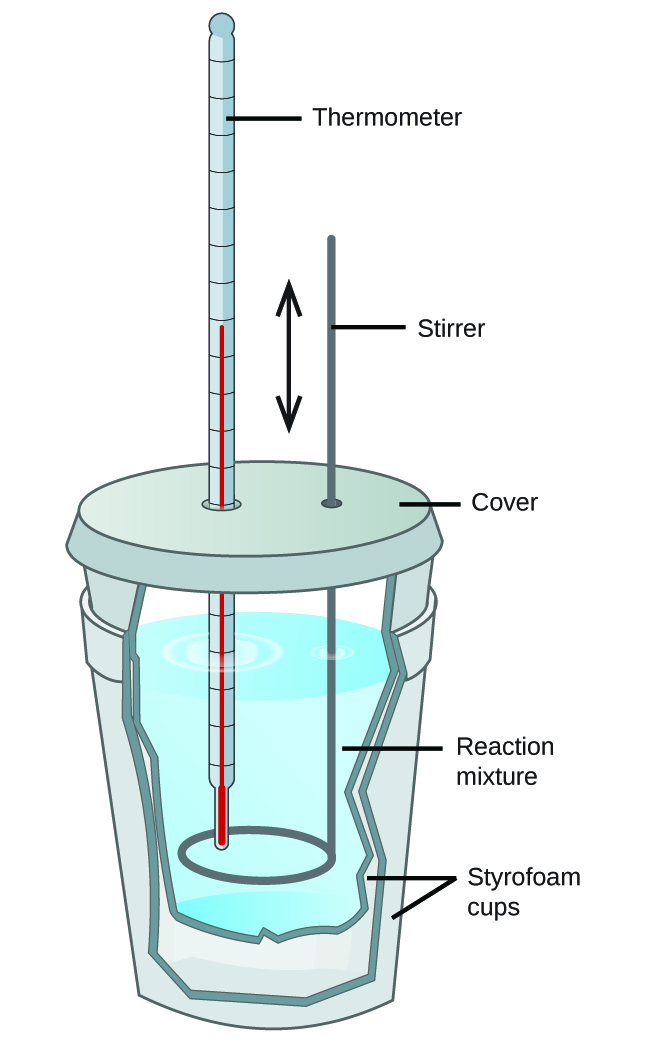
\includegraphics[width=0.2\linewidth]{CoffeeCupCalorimeter}
	\caption[Coffee Cup Calorimeter]{Coffee Cup Calorimeter}
	\label{fig:coffeecupcalorimeter}
\end{figure}

Let us now calculate the changes in the inner energies of the various subsystems. Our primary system - the system in which the reaction takes place - undergoes a change in energy given by
$$
dU = d(H - PV) =  dH - d(PV) = dH - P dV
$$
where we have used the definition of the enthalpy and the fact that the process takes place at constant pressure, so that $dP = 0$. Let now $Q$ denote the amount of energy transferred as heat from our system into the heat sink. Then the inner energy of the heat sink increases by $Q$, i.e.
$$
dU_{HS} = Q
$$
as the heat sink is otherwise isolated so that no mechanical or chemical work is done on it. Similarly, the energy of the pressure reservoir increases by $P dV$
$$
dU_{PR} = P dV
$$
Thus the overall energy changes by
\begin{align*}
dU_{tot} &= dU + dU_{HS} + dU_{PR} \\
&= (dH - P dV) + Q + P dV = dH + Q
\end{align*}
However, as we assume that the overall system is isolated towards the environment, the total change of energy is zero. Thus
$$
0 = dH + Q
$$
or
$$
Q = - dH
$$ 
This shows that the {\em change in enthalpy is (minus) the heat released by a process at constant pressure}. If the change of enthalpy is negative, the amount of heat released is positive, so we have an {\em exothermic reaction}. If the change of enthalpy is positive, the reaction consumes heat and is {\em endothermic}.

One of the reasons why the enthalpy is so useful is that it is - by construction - a function on the configuration space. Thus the change in enthalpy depends only on the final and the initial state of the system (which is in general not true for heat as the heat transfer is given by the one-form $T dS$ which is not exact and therefore depends on the process, i.e. on the path in configuration space representing the process). To see why this is useful in practice, let us consider an example. Say we wanted to calculate the change in enthalpy of the reaction 
$$
A \longrightarrow B
$$ 
and suppose further that we already knew the enthalpy changes for the reactions
$$
A \longrightarrow C 
$$
and 
$$
C \longrightarrow B
$$
Now each of the reaction reactants and products that we have abbreviated with $A, B, C$ are states of our system - a certain amount of molecules of the respective type dissolved in water (as long as we stick to some standard conditions, which are conventially chosen to be a pressure of 1 bar and a temperature of 298 K). Thus each of them has a certain value of the enthalpy, and the change in enthalpy is simply the difference of the enthalpy after and before the reaction took place. This implies, however, that we can simply calculate enthalpy changes of new reactions by adding up enthalpy changes of existing reactions in the obvious way, specifically
\begin{align*}
\Delta H_{A \longrightarrow B } &= H_B - H_A \\
\Delta H_{A \longrightarrow C } &= H_C - H_A \\
\Delta H_{C \longrightarrow B } &= H_B - H_C \\
\end{align*}
and therefore
$$
\Delta H_{A \longrightarrow B } = \Delta H_{A \longrightarrow C } + \Delta H_{C \longrightarrow B }
$$
This fact is known as Hess`s law of enthalpies and allows us to calculate the changes of enthalpies for complex reactions by piercing together the enthalpy changes for simpler reactions that we might already have measured and tabulated.

Finally, let us relate the enthalpy with the Gibbs free energy that we have discussed in the previous section. By definition
$$
G = U + pV - TS = H - TS
$$
so that
$$
dG = dH - d(TS) = dH - T dS
$$
at constant temperature. Thus if the enthalpy change of a reaction is negative, i.e. the reaction is exothermic, and the entropy change of the reaction is positive, the reaction will take place spontaneously (reducing the enthalpy and increasing the entropy at the same time). If a reaction is endothermic and the entropy change is negative, the Gibbs energy is positive, so that the reaction will not take place. If, however, the enthalpy change is negative but the entropy change is negative as well, it depends on the temperature whether the reaction takes place spontaneously (note, however, that both enthalpy change and Gibbs energy depend on the temperature as well, so the condition for a negative Gibbs energy change	 is not as simple as our notation might indicate).

We close this section by discussing another relation between the Gibbs free energy and the enthalpy known as the van't Hoff equation. Recall that with the convention typically used in chemistry textbooks, the relation between the equilibrium constant and the Gibbs free energy change for the reaction at constant pressure and temperature of one mole of substance reads
$$
K = \exp (- \frac{\Delta G}{R T})
$$
or
$$
\ln K = - \frac{\Delta G}{R T}
$$
As $G = H - TS$, this is the same as
$$
\ln K = - \frac{\Delta H}{R T} + \frac{\Delta S}{R}
$$
where $\Delta S$ is the entropy change of the reaction and $\Delta H$ is the change of enthalpy. Of course both quantities depend on the temperature at which the reaction takes place. However, let us ignore this dependency for a moment and assume that these quantities are - for small changes in the temperature - independent of the temperature. Then we can take the derivative with respect to $T$ and obtain
$$
\frac{d}{dT} \ln K =  \frac{\Delta H}{R T^2} 
$$
This equation that approximates how the equilibrium constant depends on the temperature is known as van't Hoff equation. Alternatively, we could write this as
$$
\ln \frac{K(T_2)}{K(T_1)} =  \frac{\Delta H}{R} (\frac{1}{T_1} - \frac{1}{T_2})
$$
Note that for an endothermic reaction, this predicts that when we increase the temperature, the equilibrium is moved to the right, and for an exothermic reaction the equilibrium is moved to the left. 

The van't Hoff equation has an interesting graphical interpretation. Suppose that we could measure the equilibrium constant for different temperatures (close enough to the standard temperature that our approximation does not break down) and plot the natural logarithm of $K$ versus the inverse temperature $T^{-1}$. Then the van't Hoff equation tells us that the result will be a line. The slope of this line multiplied by $R$ is minus the enthalpy change of the reaction, while the point value at which it intersects the y-axis multiplied by $R$ gives the entropy change of the reaction. This plot is known as {\em van't Hoff plot}, and can be used to determine enthalpy change and entropy change without using a calorimeter.

\section{Appendix - the Gibbs-Duhem equation}

One of the postulates of thermodynamics is that the entropy is an extensive quantity: when we double the size of a system (i.e. its volume, its number of particles and its internal energy) the entropy will double. Technically, this comes down to the requirements that
$$
S(\lambda U, \lambda N, \lambda V ) = \lambda S(U, N, V)
$$
for all scaling factors $\lambda$. Functions with this property are called homogenous and it turns out that these functions have a very special form.

\begin{defn}
A function $f \colon \R^n \rightarrow \R$ is called {\em homogenous} when the relation
$$
f(\lambda x ) = \lambda f(x)
$$
holds for all $\lambda \geq 0$ and all $x \in \R^n$.
\end{defn}


\begin{thm}[Eulers theorem on homogenous functions]\label{thm:euler}
	If $f \colon \R^n \rightarrow \R$ is smooth and homogenous, then for every point $x$, the relation
	$$
	f(x) = \sum_{i=1}^n (\partial_i f)(x) x_i
	$$
	holds. Moreover, the partial derivatives $\partial_i f$ have the property that $(\partial_i f)(\lambda x) = (\partial_i f)(x)$, i.e. they are constant along rays.
\end{thm}


\begin{proof}
Suppose we are given an arbitrary but fixed point $x$. Consider the function $g$ defined on $\R$ by
$$
g(\lambda) = f(\lambda x) - \lambda f(x)
$$
As $f$ is homogenous, this function is zero on $[0, \infty)$, so its derivative on $(0, \infty)$ is as well. On the other hand, we can use the chain rule to see that
$$
0 = g'(\lambda) = \sum_i  (\partial_i f)(\lambda x) x_i - f(x)
$$
Setting $\lambda = 1$ yields our desired result. To prove our second statement, note that, by definition,
$$
(\partial_i f)(\lambda x) = \frac{d}{dt}|_{t=0} f(\lambda x + t e_i)
$$
which we can write as
$$
\frac{d}{dt}|_{t=0} f(\lambda (x + u e_i)) = \lambda \frac{d}{dt}|_{t=0} f(x + u e_i)
$$
with the substitution $u = \lambda^{-1} t$. As $dt = \lambda du$, the $\lambda$ term cancels and we find that 
$$
(\partial_i f)(\lambda x) = \frac{d}{du}|_{t=0} f(x + u e_i) = (\partial_i f)( x)
$$
as claimed.
\end{proof}

Let us now apply this theorem to the entropy, which is an extensive quantity (under the assumption that our system is homogenous). We obtain
$$
S(U, V, N) = \frac{\partial S}{\partial U} U + \frac{\partial S}{\partial V} V + \frac{\partial S}{\partial N} N
$$
Using the identifications of the various partial derivatives with temperature, pressure and chemical potential, this turns into
$$
S(U, V, N) = \frac{1}{T} U + \frac{1}{T} P V - \frac{1}{T} \mu N 
$$
Multiplying this by the temperature and rearranging yields
$$
U(S, V, N) = TS - PV + \mu N
$$
With more than one type of particles involved, this equation becomes
$$
U(S, V, N) = TS - PV + \sum_i \mu_i N_i
$$
Using this, we can now easily find an expression for the Gibbs free energy. As 
$$
G = U + PV - TS
$$
we see that
$$
G(T, P, N_i) = \sum_i \mu_i N_i
$$
which is an amazingly simple expression (which, however, has some hidden complexities as the $\mu_i$ will in general depend on parameters, i.e. $\mu_i$ might even depend on $N_j$ as the example of the formula for the chemical potential in a dilute solution nicely illustrates). 

To see yet another implication of the homogenous function theorem, let us take the derivative of our expression for $U$. We obtain
\begin{align*}
dU &= d(TS - PV) + \sum_i d(\mu_i N_i) \\
&= S dT + T dS - P dV - V dP + \sum_i \mu_i dN_i + \sum_i N_i d\mu_i 
\end{align*}
On the other hand, we know by the fundamental relation of thermodynamics that
$$
dU = T dS - P dV  + \sum_i \mu_i dN_i 
$$
Collecting the remaining terms yields
$$
0 = S dT  - V dP + \sum_i N_i d\mu_i 
$$
or, rearranged
$$
- S dT  + V dP = \sum_i N_i d\mu_i 
$$
This is the famous {\em Gibbs-Duhem equation} that states that the intrinsic thermodynamical variables are not fully independent. It implies in particular that for a quasi-static process at constant pressure and temperature, the derivatives of the chemical potentials are related by
$$
0 = \sum_i N_i d\mu_i 
$$


%%%%%%%%%%%%%%%%%%%%%%%%%%%%%%%%%%%%%%%%%%%%%%
%% Bibliography
%%%%%%%%%%%%%%%%%%%%%%%%%%%%%%%%%%%%%%%%%%%%%%

\begin{thebibliography}{9}
	
\bibitem{Bauer}
H.~Bauer,
{\em Wahrscheinlichkeitstheorie},
de Gruyter, Berlin, New York 1991
	
\bibitem{Klenke}
A.~Klenke,
{\em Probability theory}
Springer, London 2008


\bibitem{Shannon}
C.E.~Shannon,
{\em A mathematical theory of communication}, 
The Bell System Technical Journal {\em Vol. 27}, pp. 379--423, pp. 623--656, July, October 1948



\bibitem{Callen}
H.B.~Callen,
{\em Thermodynamics and an introduction to Thermostatistics},
Wiley, New York 1985


\bibitem{Schroeder}
D.V.~Schroeder,
{\em An introduction to thermal physics},
Addison-Wesley, San Francisco 2000

\bibitem{Sweden}
Robert H.~Sweden,
{\em An Introduction to Statistical Mechanics and Thermodynamics}, Oxford University Press 2012

\bibitem{Petrucci}
R.H.~Petrucci et al., 
{\em General chemistry - principles and modern applications}, 11th edition, Pearson, Toronto 2017

\bibitem{openstax}
OpenStax, {\em Chemistry 2e}, available at \url{https://openstax.org/details/books/chemistry-2e}

\bibitem{Tables}
National Bureau of Standards, {\em The NBS table of chemical thermodynamical properties}, Journal of Physical and Chemical Reference Data, Volume 11 (1982), Supplement No. 2

\end{thebibliography}
\end{document}


